In this chapter, we focus on the quasi-2D Coulomb systems in uniform dielectric media, and introduce a fast algorithm named the random batch sum-of-exponentials Ewald2D (RBSE2D) method, which reaches an optimal time complexity of $O(N)$ for the force calculation and can easily handle the systems with large aspect ratios.

\section{Sum-of-exponentials Ewald2D method} \label{sec:method}

In this section, we introduce a novel summation method by using the SOE approximation in evaluating $\xi^{\pm}(h,z)$ and $\partial_{z}\xi^{\pm}(h,z)$. 
This method significantly reduces the overall complexity of Ewald2D to $O(N^{7/5})$ without compromising accuracy. 
Error and complexity analyses are also provided.

%\subsection{The sum-of-exponentials method}
We first give a brief overview of the SOE kernel approximation method.  
For a given precision $\varepsilon$, the objective of an SOE approximation is to find suitable weights $w_l$ and exponents $s_l$ such that~$\forall x \in \mathbb{R}$, the following inequality holds:
\begin{equation}\label{eq::SOE1}
	\left|f(x)-\sum_{l=1}^M w_l e^{-s_l|x|}\right|\leq \varepsilon,
\end{equation}
where $M$ is the number of exponentials. 
Various efforts have been made in literature to approximate different kernel functions using SOE, as documented in works such as~\cite{wiscombe1977exponential, evans1980least, jiang2008efficient, beylkin2005approximation, beylkin2010approximation}.
For instance, the Gaussian kernel $f(x)=e^{-x^2}$ is widely celebrated and plays a crucial role in numerical PDEs~\cite{weideman2010improved,wang2018adaptive}, and is particularly relevant for the purpose of this work. 
The SOE approximation for Gaussians can be understood as discretizing its inverse Laplace transform representation, denoted as
\begin{equation}\label{eq:inverse_laplace}
	e^{-x^2} = \frac{1}{2 \pi \m{i}} \int_{\Gamma} e^{z} \sqrt{\frac{\pi}{z}} e^{-\sqrt{z}\abs{x}} dz\;,
\end{equation}
where $\Gamma$ is a suitably chosen contour. 

% Discretization of the integral in Eq.~\eqref{eq:inverse_laplace} leads to an SOE approximation as given in Eq.~\eqref{eq::SOE1}.
To achieve higher accuracy, several classes of contours have been studied, such as Talbot contours~\cite{lin2004numerical}, parabolic contours~\cite{makarov2000exponentially}, and hyperbolic contours~\cite{lopez2004numerical}. 
An alternative approach is developed by Trefethen, \emph{et al.}~\cite{trefethen2006talbot}, where a sum-of-poles expansion is constructed by the best supremum-norm rational approximants.
A comprehensive review of these techniques has been discussed by Jiang and Greengard~\cite{jiang2021approximating}.
Since the Laplace transform of an SOE is a sum-of-poles expansion~\cite{greengard2018anisotropic}, the model reduction (MR) technique can be employed to further reduce the number of exponentials $M$ while achieving a specified accuracy~$\eps$.
When combining with the MR, convergence rates at $\mathcal{O}(6^{-M}) \sim \mathcal{O}(7^{-M})$ can be achieved~\cite{jiang2021approximating}.

Additionally, kernel-independent SOE methods have been developed, such as the black-box method~\cite{greengard2018anisotropic} and Vall\'ee-Poussin model reduction (VPMR) method~\cite{gao2021kernelindependent}. 
Specially, the VPMR method integrates the flexibility of Vall\'ee-Poussin sums into the MR technique, demonstrating the highest convergence rate of $\mathcal{O}(9^{-M})$ in constructing SOE approximation for Gaussians. 
This method is also bandwidth-controllable and uniformly convergent~\cite{AAMM-13-1126}. 
Due to these advantages, we will utilize the VPMR as the SOE construction tool in all the numerical experiments throughout this paper.


% Moreover, various efforts have been made in the literature to approximate different kernel functions using SOE, as documented in works such as~\cite{wiscombe1977exponential, evans1980least, jiang2008efficient, beylkin2005approximation, beylkin2010approximation}. We do not intend to present a comprehensive review of these algorithms here and refer the reader to these references for further details.

%\begin{rmk}
%It is worth noting that the existing methods for %constructing a sum-of-Gaussians approximation can be %easily extended to constructing an SOE by %incorporating a change of variable $x=\sqrt{t}$.
%\end{rmk}

\subsection{SOE approximations of $\xi^{\pm}(h,z)$} \label{subsec::SOEapp}

To start with, we introduce a useful identity which is a special case of the Laplace transform~(\cite{oberhettinger2012tables}, pp.~374-375; \cite{myint2007linear}, pp.~688). 
\begin{lem}
	Suppose that $a$, $b$, and $c$ are three complex parameters where the real part of $a$ satisfies $\mathscr{R}(a)>0$. For an arbitrary real variable $x$, the following identity holds:
	\begin{equation}\label{eq::identity}
		\int_{x}^{\infty} e^{-(at^2+2bt+c)}dt=\frac{1}{2}\sqrt{\frac{\pi}{a}}e^{(b^2-ac)/a}\erfc\left(\sqrt{a}x+\frac{b}{\sqrt{a}}\right).
	\end{equation}
\end{lem}

Substituting $a=\alpha^2$, $b=h/2$, $c=0$, $x=\pm z$ into Eq.~\eqref{eq::identity} yields the integral representations of $\xi^{\pm}(h,z)$:
\begin{equation}\label{eq::xi20}
	\xi^{\pm}(h,z) = \frac{2\alpha}{\sqrt{\pi}}e^{-h^2/(4\alpha^2)}e^{\pm hz}\int_{\pm z}^{\infty}e^{-\alpha^2t^2-ht} dt \;.
\end{equation}
We then approximate the Gaussian factor $e^{-\alpha^2t^2}$ in the integrand of Eq.~\eqref{eq::xi20} by an $M$-term SOE on the whole real axis, as
\begin{equation}\label{eq::xi21}
	e^{-\alpha^2 t^2} \approx \sum_{l = 1}^M w_{l} e^{ - s_{l} \alpha \abs{t}}\;.
\end{equation}
% That is, for a prescribed precision $\varepsilon$ and a real variable $x$, we assume that
% \begin{equation}\label{eq::SOE1}
	% \left|e^{-x^2}-\sum_{\ell=1}^M w_l e^{-s_l|x|}\right|\leq \varepsilon
	% \end{equation}
% exists where $M$ is the number of exponentials, $w_l$ denotes the weights, and $s_l$ denotes the exponents. 
Inserting Eq.~\eqref{eq::xi21} into Eq.~\eqref{eq::xi20} results in an approximation to $\xi^{\pm}(h,z)$:
\begin{equation}\label{eq::xi_M_int}
	\xi_{M}^{\pm}(h, z) := \frac{2\alpha}{\sqrt{\pi}} e^{-h^2/(4\alpha^2)} e^{\pm hz} \int_{\pm z}^{\infty} \sum_{l = 1}^M w_{l} e^{ - s_{l} \alpha \abs{t}} e^{-ht} dt \;.
\end{equation}
The integral can be calculated analytically (with $\alpha, z > 0$), yielding 
\begin{equation}\label{eq::plus}
	\xi_M^{+}(h,z) = \frac{2 \alpha}{\sqrt{\pi}} e^{-h^2/(4 \alpha^2)} \sum_{l = 1}^M w_l\frac{e^{- \alpha s_l z}}{\alpha s_l + h } 
\end{equation}
and
\begin{equation}\label{eq::minus}
	\xi_{M}^{-}(h, z) = \frac{2 \alpha}{\sqrt{\pi}} e^{-h^2/(4 \alpha^2)} \sum_{l = 1}^M w_l \left[ - \frac{e^{-\alpha s_l z}}{\alpha s_l - h} + \frac{2\alpha s_l e^{- hz}} {(\alpha s_l)^2 - h^2} \right] \;.
\end{equation}
Similarly, one can also obtain the approximation of~$\partial_z \xi^{\pm}(h,z)$, given by
\begin{equation}\label{eq::dz_plus}
	\partial_z \xi_{M}^{+}(h, z) := - \frac{2 \alpha^2 }{\sqrt{\pi}} e^{-h^2/(4 \alpha^2)} \sum_{l = 1}^M w_l s_l \frac{e^{- \alpha s_l z}}{\alpha s_l + h } 
\end{equation}
and
\begin{equation}\label{eq::dz_minus}
	\partial_z \xi_{M}^{-}(h, z) := - \frac{2 \alpha^2}{\sqrt{\pi}} e^{-h^2/(4 \alpha^2)} \sum_{l = 1}^M w_l s_l \left[ - \frac{e^{-\alpha s_lz}}{\alpha s_l - h} + \frac{2 h e^{- hz}} {(\alpha s_l )^2 - h^2} \right] \;.
\end{equation}
The approximation error, which relies on the prescribed precision $\varepsilon$ of the SOE, also has spectral convergence in $h$.
This is summarized in Theorem \ref{thm:error_xi}.

\begin{thm}\label{thm:error_xi}
	Given an $M$-term SOE expansion for the Gaussian kernel $f(x)=e^{-\alpha^2x^2}$ satisfying Eq.~\eqref{eq::SOE1}, the approximation of~$\xi^{\pm}$ derived from Eqs.~\eqref{eq::xi20}-\eqref{eq::minus} has a global error bound
	\begin{equation}\label{eq::bound_xi}
		\abs{\xi^{\pm}(h,z) - \xi_{M}^{\pm}(h, z)} \leq \frac{2 \alpha e^{-h^2/(4 \alpha^2)}}{\sqrt{\pi} h} \varepsilon\;,
	\end{equation}
	and for the approximation of~$\partial_z \xi^{\pm}$ using Eqs.~\eqref{eq::dz_plus}-\eqref{eq::dz_minus}, the error bound is given by
	\begin{equation}\label{eq::bound_dz_xi}
		\abs{\partial_z \xi^{\pm}(h,z) - \partial_z \xi_{M}^{\pm}(h, z)} \leq \frac{4 \alpha e^{-h^2/(4 \alpha^2)}}{\sqrt{\pi}} \varepsilon\;,
	\end{equation}
	which is independent of $z$ and decays rapidly with $h$.
\end{thm}

\begin{proof}
	To prove Eq.~\eqref{eq::bound_xi}, one can directly subtract Eq.~\eqref{eq::xi_M_int} from  Eq.~\eqref{eq::xi20} to obtain:
	\begin{equation}
		\begin{split}
			&\abs{\xi^{\pm}(h, z) - \xi_{M}^{\pm}(h, z)}\\
			\leq & \frac{2 \alpha}{\sqrt{\pi}} e^{-h^2/(4 \alpha^2)} \int_{\pm z}^\infty e^{\pm hz - h t} \abs{e^{-\alpha^2 t^2} - \sum_{l = 1}^M w_l e^{-\alpha s_l\abs{t}} } dt \\
			\leq & \frac{2 \alpha}{\sqrt{\pi}} e^{ - h^2/(4 \alpha^2)} \varepsilon \int_{\pm z}^\infty e^{\pm hz - h t} dt \\
			= & \frac{2 \alpha e^{-h^2/(4 \alpha^2)}}{\sqrt{\pi} h} \varepsilon\;,
		\end{split}
	\end{equation}
	where from the second to the third line, one uses the boundness of SOE approximation error, i.e., Eq.~\eqref{eq::SOE1}.
	For the approximation error of $\partial_z\xi^{\pm}$, the proof is similar. One can subtract the $z$-derivative of Eq.~\eqref{eq::xi_M_int} from the $z$-derivative of Eq.~\eqref{eq::xi20} to obtain
	\begin{equation}
	\begin{split}
	& \abs{\partial_z \xi^{\pm}(h, z) - \partial_z \xi_{M}^{\pm}(h, z)}\\
	\leq & \frac{2 \alpha}{\sqrt{\pi}} e^{-h^2/(4 \alpha^2)} \left( \int_{\pm z}^\infty h e^{\pm hz - h t} \abs{e^{-\alpha^2 t^2} - \sum_{l = 1}^M w_l e^{-\alpha s_l\abs{t}} } dt + \abs{e^{-\alpha^2 z^2} - \sum_{l = 1}^M w_l e^{-\alpha s_l\abs{z}} } \right)\\
	\leq & \frac{2 \alpha}{\sqrt{\pi}} e^{ - h^2/(4 \alpha^2)} \varepsilon \left( h \int_{\pm z}^\infty e^{\pm hz - h t} dt + 1 \right) \\
	= & \frac{4 \alpha e^{-h^2/(4 \alpha^2)}}{\sqrt{\pi}} \varepsilon\;.
	\end{split}
	\end{equation}
	Again, the boundness of the SOE approximation error is used in the proof, i.e., from the second to the third line.
\end{proof}


For the $\V 0$-th frequency term Eq.~\eqref{eq:phil0} consisting of $\erf(\cdot)$ and Gaussian functions, a similar approach can be employed to construct the corresponding SOE expansions. One has
\begin{equation}\label{eq:SOErf}
	\begin{split}
		\erf(\alpha z)\approx \frac{2}{\sqrt{\pi}} \int_0^{\alpha z} \sum_{l = 1}^M w_l e^{-s_l t} dt= \frac{2}{\sqrt{\pi}} \sum_{l = 1}^M \frac{w_l}{s_l} (1 - e^{- \alpha s_l z})\;.
	\end{split}
\end{equation}
One can prove that
\begin{equation}\label{eq::erfSOE}
	\left|\erf(\alpha z)-\frac{2}{\sqrt{\pi}} \sum_{l = 1}^M \frac{w_l}{s_l} (1 - e^{- \alpha s_l z})\right|\leq \frac{2\alpha H}{\sqrt{\pi}}\varepsilon\;,
\end{equation}
where one assumes that $z\in[0, H]$, as for quasi-2D systems all particles are confined within a narrow region in $z$. 

The advantages and novelty of our SOE approach are summarized as follows.
Firstly, Theorem~\ref{thm:error_xi} demonstrates that the approximation error of our SOE method is uniformly controlled in $z$ and decays exponentially in $k$. Secondly, the resulting approximation $\xi_{M}^{\pm}$ is well-conditioned, thus addressing the issue of catastrophic error cancellation when evaluating $\xi^{\pm}$. 
Achieving these properties are crucial for the subsequent algorithm design.

\begin{rmk}
	The choice of SOE approximation is not unique. Instead of approximating the Gaussian factor in the integrand with an SOE, a more directforward approach might be approximating the complementary error function in~$\xi^{\pm}$ using an SOE. 
	Unfortunately, this will introduce an error proportional to~$e^{hz} \varepsilon$, which grows exponentially with~$h$, resulting in a much larger numerical error in the Fourier space summation for the long-range components of Coulomb energy and forces.
\end{rmk}	


\begin{figure}[ht] 
	\centering
	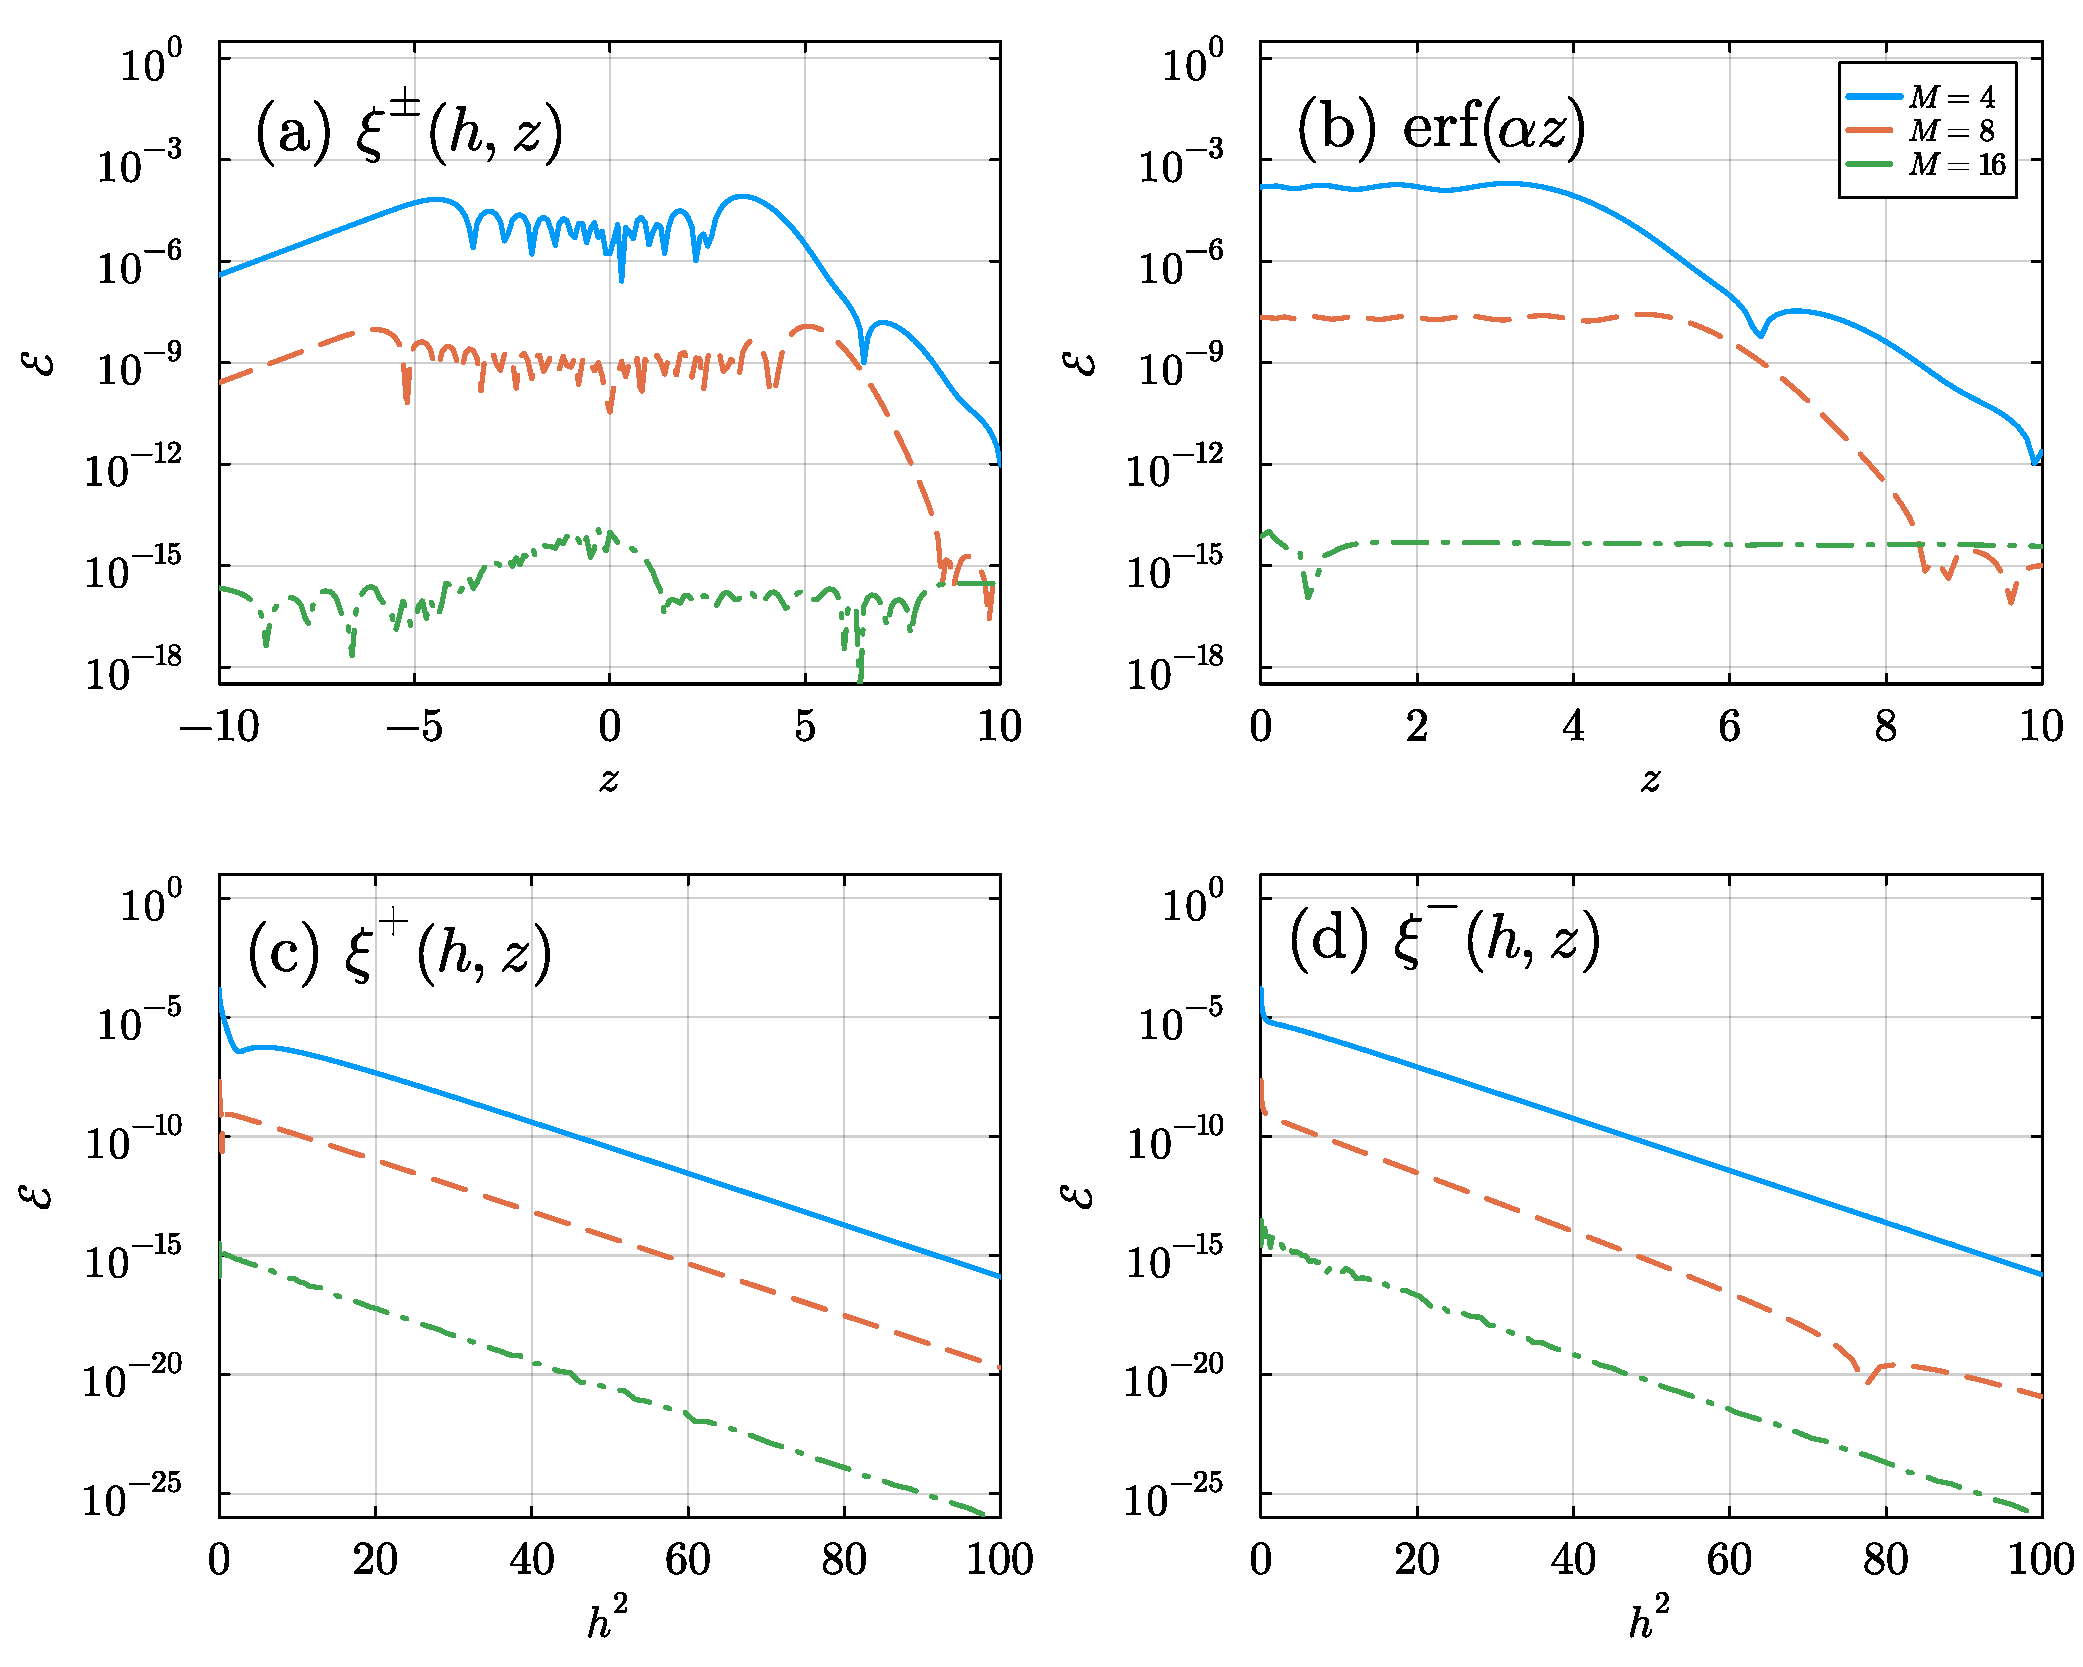
\includegraphics[width=\textwidth]{figs/fig_error_Uxi.pdf}
	\caption{
		The absolute error of the SOE expansion for (a) $\xi^{\pm}(h,z)$ and (b) $\erf(\alpha z)$ is plotted as a function of $z$, while fixing $h=\alpha=1$; absolute error of the SOE expansion of (c) $\xi^{+}(h,z)$ and (d) $\xi^{-}(h,z)$ as a function of $h^2$, while fixing $z=1$.
		Data are presented for SOEs with varying numbers of exponentials, $M=4,$ 8 and 16.
	}
	\label{fig:error_SOE}
\end{figure}

% Analogously, one can approximate the corresponding $z$-derivatives, $\partial_z \xi^{\pm}(k,z)$ and $\partial_z \erf(\alpha z)$ via SOE approximations, which is important in force calculations. The resulting expressions, error estimates, as well as numerical validations are provided in Appendix~\ref{app:dz_ksi}.
% Several advantages in using SOE approximation to reformulate Ewald2D will be further demonstrated, as we proceed to the next section. 
% Both $\xi_{M}^{+}(k, z)$ and $\xi_{M}^{-}(k, z)$ take the form of the SOE with respect to $z$. 
% Comparing with their original forms Eq.~\eqref{eq::9}, the advantages of the SOE-based reformulation are threefold:
% \begin{itemize}
	%     \item[1.] The translational invariance of the exponential function enables variable separation in non-periodic dimension. 
	%     \item[2.] By eliminating all terms of the form $e^{kz}$, the issue of catastrophic error cancellation is effectively addressed.
	%     \item[3.] Similar to the fully-periodic case~\cite{Ewald1921AnnPhys,jin2021random}, the explicit decay factor $e^{-k^2/(4\alpha^2)}$ allows for the construction of fast algorithms to accelerate computations in the first two periodic dimensions. 
	% \end{itemize}
% These advantages will be further demonstrated.

\subsection{SOEwald2D summation and its fast evaluation}\label{subsec::reforEwald2}
In this section, we derive the SOE-reformulated Ewald2D (SOEwald2D) summation, and the corresponding fast evaluation scheme. 
Let us first consider the contribution of the $\V{h}$-th mode $(\V h \neq \V{0})$ to the long-range interaction energy, denoted as $U_{\ell}^{\V{h}}$, which can be written in the following pairwise summation form 
\begin{equation}\label{eq::pairssum8}
	\begin{split}
		U_{\ell}^{\V{h}} = \frac{1}{2} \sum_{i = 1}^N q_{i} \phi^{\V{h}}_\ell(\V{r}_{i}) =\frac{\pi}{L_xL_y}\sum_{1\leq j<i\leq N}q_{i}q_{j} \varphi^{\bm{h}} (\bm{r}_{i},\bm{r}_{j}) + \frac{Q \pi}{h L_x L_y} \erfc\left(\frac{h}{2 \alpha}\right)\;,
	\end{split}
\end{equation}
where we define
\begin{equation}\label{eq:varphi_k}
	\varphi^{\bm{h}}(\bm{r}_{i},\bm{r}_{j}):=\frac{e^{\m{i} \V{h} \cdot \V{\rho}_{ij}}}{h} \left[\xi^{+}(h, z_{ij})+\xi^{-}(h, z_{ij})\right].
\end{equation}
Substituting the SOE approximation of $\xi^{\pm}(h,z)$ described in Eqs.~\eqref{eq::plus} and \eqref{eq::minus}, a new SOE-based formulation can be obtained, denoted as $U_{\ell,\text{SOE}}^{\V{h}}$. 
This approximation is achieved by substituting $\varphi^{\bm{h}}(\bm{r}_{i},\bm{r}_{j})$ with
\begin{equation}\label{eq::SOEphi}
	\begin{split}
		\varphi^{\bm{h}}_{\text{SOE}}(\bm{r}_{i},\bm{r}_{j}) & := \frac{e^{\m{i} \V{h} \cdot \V{\rho}_{ij}}}{h} \left[\xi^{+}_M(h, z_{ij})+\xi^{-}_M(h, z_{ij})\right]\\
		&=\frac{2\alpha e^{-h^2/(4\alpha^2)}}{\sqrt{\pi}h}e^{\m{i}\V{h} \cdot \V{\rho}_{ij}} \sum_{\ell = 1}^{M}  \frac{w_l}{\alpha^2 s_l^2 - h^2}\left( 2 \alpha s_l e^{-h z_{ij}} - 2ke^{-\alpha s_l z_{ij}}\right) \;.
	\end{split}
\end{equation}

For the $\V 0$-th mode contribution $U_{\ell}^{\V{0}}$, an SOE-based reformulation can be similarly obtained according to Eq.~\eqref{eq:SOErf}:
\begin{equation}\label{eq::Ul0SOE}
	U_{\ell,\text{SOE}}^{\bm{0}} = \frac{1}{2} \sum_{i = 1}^N q_{i} \phi^{\bm{0}}_\ell(\V{r}_{i}) = - \frac{2\pi}{L_xL_y}\sum_{1\leq j < i \leq N}q_{i}q_{j}\varphi^{\bm{0}}_{\text{SOE}}(\bm{r}_{i},\bm{r}_{j})-\frac{\pi Q}{\alpha L_xL_y},
\end{equation}
where
\begin{equation}\label{eq::32}
	\varphi^{\bm{0}}_{\text{SOE}}(\bm{r}_{i},\bm{r}_{j}):=\sum_{l=1}^{M}\frac{w_l}{\sqrt{\pi}}\left[\frac{2z_{ij}}{s_l}+\left(\frac{1}{\alpha}-\frac{2z_{ij}}{s_l}\right)e^{-\alpha s_l z_{ij}}\right].
\end{equation}

We now present an iterative approach to compute $U_{\ell,\text{SOE}}^{\V{h}}$ for each $\bm{h}$ with $\mathcal O(N)$ complexity. 
For simplicity, consider pairwise sum in the following form:
\begin{equation}\label{eq::33}
	S = \sum_{1\leq j < i \leq N} q_{i} q_{j} e^{\m{i} \V{h} \cdot \V{\rho}_{ij}} e^{ - \beta z_{ij} }\;,
\end{equation}
where $\beta$ is a parameter satisfying $\mathscr{Re}(\beta)>0$. It is clear that the pairwise sums in both $U_{\ell,\text{SOE}}^{\V{h}}$ and $U_{\ell,\text{SOE}}^{\V{0}}$ are in the form of Eq.~\eqref{eq::33}, and direct evaluation takes $\mathcal O(N^2)$ cost. 

To efficiently evaluate $S$, we initially sort the particle indices based on their $z$ coordinates, such that~$i > j \iff z_i > z_j$.
% $z_1 \leq z_2 \leq \cdots \leq z_N$. 
Subsequently, the summation can be rearranged into a separable and numerically stable form:
\begin{align}
	S &=\sum_{i = 1}^N q_{i} e^{\m{i} \bm{h}\cdot\bm{\rho}_{i}}e^{-\beta z_{i}} \sum_{j = 1}^{i - 1} q_{j} e^{-\m{i} \bm{h}\cdot\bm{\rho}_{j}}e^{\beta z_{j}} \label{eq::S0} \\ 
	&= \sum_{i = 1}^N q_{i} e^{\m{i} \bm{h}\cdot\bm{\rho}_{i}}e^{-\beta(z_{i} - z_{i - 1})}A_{i}(\beta)\;, \label{eq::S}
\end{align}
with coefficients
\begin{equation}
	A_{i}(\beta) =  \sum_{j = 1}^{i - 1} q_{j} e^{-\m{i} \bm{h}\cdot\bm{\rho}_{j}}e^{-\beta(z_{i - 1} - z_{j})}\;.
\end{equation}
Clearly, $A_1(\beta)=0,$ $A_2(\beta)=q_1e^{-\m{i} \bm{h}\cdot\bm{\rho}_1}$, and for $i\geq 3$, a recursive algorithm can be constructed to achieve $\mathcal O(N)$ complexity in computing all the coeffcients:
\begin{equation}\label{eq::35}
	A_{i}(\beta) = A_{i - 1}(\beta) e^{-\beta(z_{i - 1} - z_{i - 2})} + q_{i - 1}e^{-\m{i} \bm{h}\cdot\bm{\rho}_{i-1}}\;,\quad i = 3, \cdots, N.
\end{equation}
One can thus efficiently evaluate $S$ with another $\mathcal{O}(N)$ operations by Eq.~\eqref{eq::S} and using the computed coefficients~$\V{A}(\beta) = (A_1(\beta), ..., A_N(\beta))$. 
Consequently, the overall cost for evaluating the pairwise summation in forms of Eq.~\eqref{eq::33} is reduced to $\mathcal{O}(N)$.
Besides the iterative method discussed above, it is remarked that different fast algorithms based on SOE for 1D kernel summations have been developed~\cite{jiang2021approximating,GIMBUTAS2020815}, which can also be used under the framework described in this article for the summation in the non-periodic direction.
% The key point lies in finding an SOE that provides accurate approximations for all Fourier modes, as demonstrated in Section~\ref{subsec::SOEapp} of this paper.

\begin{rmk}
	A similar iterative evaluation strategy can be developed based on Eq.~\eqref{eq::S0} instead of Eq.~\eqref{eq::S}, which may seem more straightforward.
	However, it will lead to uncontrolled exponential terms such as $e^{\beta z_{j}}$, affecting the numerical stability.
	The same issue occurs in the original Ewald2D summation.
	In our recursive scheme, by prior sorting of all particles in $z$, it follows that  $z_{i}-z_{i-1} > 0$ and $z_{i-1} - z_{j} \geq 0$ for all $j \leq i - 1$, thus making all exponential terms in Eq.~\eqref{eq::S} with negative exponents, resolving the exponential blowup issue.
	\label{rmk::stable}
\end{rmk}



Finally, the long-range component of Coulomb interaction energy in Ewald2D summation is approximated via:
\begin{equation}\label{eq:U_l_SOE}
	U_{\ell}\approx U_{\ell,\text{SOE}} := \sum_{\bm{h}\neq \bm{0}} U_{\ell,\text{SOE}}^{\bm{h}}+U_{\ell,\text{SOE}}^{\bm{0}},
\end{equation}
where both $U_{\ell,\text{SOE}}^{\bm{h}}$ and $U_{\ell,\text{SOE}}^{\bm{0}}$ can be evaluated efficiently and accurately with linear complexity.
In MD simulations, the force exerts on the $i$-th particle, $\bm{F}_{i}$, plays a significant role in the numerical integration of Newton's equations.
One can similarly develop fast recursive algorithms to evaluate the SOE-reformulated forces,
the detailed expressions for $\bm{F}_{i}$ is summarized in \ref{app::force}.
We finally summarize the SOEwald2D  in Algorithm~\ref{alg:SOEwald2D}. Its error and complexity analysis will be discussed in the next sections.

\begin{algorithm}[ht] 
	\caption{The sum-of-exponentials Ewald2D method}
	\begin{algorithmic}[1]
		% \setstretch{1.15}
		\State \textbf{Input}: Initialize the size of the simulation box $(L_x, L_y, H)$, as well as the positions, velocities, and charges of all particles. Choose a precision requirement $\varepsilon$.  %, proceed to compute the energy defined in Eq.~\eqref{eq:U} along with its corresponding gradient.
		
		\State \textbf{Precomputation stage}: Determine Ewald splitting parameters $\alpha$ and $s$ according to Eq.~\eqref{eq:trunction_error}. Generate real and Fourier space cutoffs by $r_c=s/\alpha$ and $k_c=2s\alpha$, respectively. Construct the SOE approximations of $\xi^{\pm}(h,z)$ and $\erf(\alpha z)$ following Section~\ref{subsec::SOEapp}.
		
		\Procedure\textnormal{SOEwald2D}{}   
		\State Sort all the particles according to their $z$ coordinates, as $z_1 < z_2 < \cdots < z_N$.
		\State Compute~$U_{\ell,\text{SOE}}^{\bm{h}}$ for $|\bm{h}|\leq k_c$ as well as $U_{\ell,\text{SOE}}^{\bm{0}}$ according to Section~\ref{subsec::reforEwald2}. 
		% \State Compute $U_{\text{self}}$ and $U_{\text{p-s}}$ according to Eqs.~\eqref{eq::self} and \eqref{eq::phiionwall}, respectively.
		\State Compute~$U_{s}$ by direct truncation in real space according to Eq.~\eqref{eq:phi_s} with cutoff $r_c$. %\Comment{short-range part}
		\State Compute $U_{\text{self}}$ according to Eqs.~\eqref{eq::self}.
		\State Compute $U = \sum_{|\bm{h}|\leq k_c} U_{\ell, \text{SOE}}^{\bm{h}} + U_{\ell,\text{SOE}}^{\bm{0}} - U_{\text{self}} + U_{s} + U_{\text{p-s}}$.
		\State Compute forces $\bm{F}_{i}$ using a similar procedure as that of $U$.
		\EndProcedure
		
		\State \textbf{Output}: Total electrostatic energy $U$ and forces $\bm{F}_{i}$.
		
	\end{algorithmic}\label{alg:SOEwald2D}
\end{algorithm}

\subsection{Error analysis for the SOEwald2D algorithm}\label{subsec::errSOEwald2D}
Here we derive error estimates for the SOEwald2D summation. 
The total error in the interaction energy $U$ consists of the truncation error and the SOE approximation error:
\begin{equation}
	\mathscr{E}_{U} := \mathscr{E}_{U_{s}}(r_c, \alpha) + \mathscr{E}_{U_{\ell}}(r_c, \alpha) + \sum_{\bm{k}\neq\bm{0}}\mathscr{E}_{U_{\ell},\text{SOE}}^{ \bm{h}} + \mathscr{E}_{U_{\ell},\text{SOE}}^{\bm{0}}\;,
\end{equation}
where the first two terms are the truncation error of Ewald2D summation and have already been provided in Proposition~\ref{prop::2.12}. 
The remainder two terms are the error due to the SOE approximation for the Fourier space components, where
\begin{equation}
	\mathscr{E}_{U_{\ell},\text{SOE}}^{\bm{h}}:=U_{\ell}^{\bm{h}}-U_{\ell,\text{SOE}}^{\bm{h}},\quad \text{and}\quad \mathscr{E}_{U_{\ell},\text{SOE}}^{\bm{0}}:=U_{\ell}^{\bm{0}}- U_{\ell,\text{SOE}}^{\bm{0}}.
\end{equation}
Theorem~\ref{thm:SOE_error} provides  upper bound error estimates, when the Debye-H$\ddot{\text{u}}$ckel (DH) theory is assumed (see~\cite{levin2002electrostatic}, and also~\ref{app::Debye}) to approximate the charge distribution at equilibrium.

\begin{thm}
	\label{thm:SOE_error}
	Given a set of SOE parameters $w_l$ and $s_l$ satisfying Eq.~\eqref{eq::SOE1} and a charge distribution satisfying the DH theory, the SOE approximation error for the Fourier component of interaction energy satisfies:
	\begin{equation}\sum_{\bm{h}\neq\bm{0}}\mathscr{E}_{U_{\ell},\text{SOE}}^{\bm{h}} \leq \frac{2 \lambda_D^2 \alpha^3Q}{\sqrt{\pi}}\varepsilon,
		\quad \text{and} \quad
		\mathscr{E}_{U_{\ell},\text{SOE}}^{\bm{0}} \leq \frac{\sqrt{\pi} \lambda_D^2 (1+2\alpha^2H)Q}{\alpha L_xL_y}\varepsilon,
		\label{eq::51}
	\end{equation}
	respectively, where $\lambda_D$ is the Debye length of the Coulomb system. 
\end{thm}

\begin{proof}
	By definitions of $U_{\ell}^{\bm{h}}$ and $U_{\ell,\text{SOE}}^{\bm{h}}$, one has
	\begin{equation}\label{eq::42}
		U_{\ell}^{\bm{h}}-U_{\ell,\text{SOE}}^{\bm{h}}= \frac{\pi}{2 L_xL_y}\sum_{i=1}^{N}\sum_{j\neq i}q_{i}q_{j}\frac{e^{\m{i} \bm{h}\cdot\bm{\rho}_{ij}}}{h}\mathscr{E}_{\xi^{\pm}},
	\end{equation}
	where 
	\begin{equation}\label{eq::44}
		\mathscr{E}_{\xi^{\pm}} := \abs{\xi^{+}(h,z_{ij})-\xi_{M}^{+}(h,z_{ij})} + \abs{\xi^{-}(h,z_{ij})-\xi_{M}^{-}(h,z_{ij})}\;,
	\end{equation}
	By Theorem~\ref{thm:error_xi}, one has
	\begin{equation}
		|\mathscr{E}_{\xi^{\pm}}|\leq\frac{4\alpha e^{-h^2/(4\alpha^2)}}{\sqrt{\pi}h}\varepsilon\;.
	\end{equation}
	Substituting Eq.~\eqref{eq::44} into Eq.~\eqref{eq::42} and using the DH approximation, one gets
	\begin{equation}\label{eq::47}
		\begin{split}   
			\left| \mathscr{E}_{U_{\ell},\text{SOE}}^{\bm{h}} \right| \leq \frac{2\sqrt{\pi} \lambda_D^2 \alpha Q}{L_x L_y} \frac{e^{-h^2 / (4\alpha^2)}}{h^2} \varepsilon.
		\end{split}
	\end{equation}
	To adequately consider the error in Fourier space, the thermodynamic limit is commonly considered~\cite{kolafa1992cutoff,deserno1998mesh}, wherein the sum over wave vectors is replaced by an integral over $\bm{h}$:
	\begin{equation}\label{eq::integral2}
		\sum_{\bm{h}\neq\bm{0}}\approx \frac{L_xL_y}{(2\pi)^2}\int_{\frac{2\pi}{L}}^{\infty}h dh\int_{0}^{2\pi}d\theta,
	\end{equation}
	where $(h,\theta)$ are the polar coordinates and $L=\max\{L_x,L_y\}$. It then follows that
	\begin{equation}
		\sum_{\bm{h}\neq\bm{0}}\mathscr{E}_{U_{\ell},\text{SOE}}^{ \bm{h}}\leq \frac{2\lambda_D^2\alpha^3Q}{\sqrt{\pi}}\varepsilon.
	\end{equation}
	Finally, recalling the SOE approximation errors of $\erf(\cdot)$ and Gaussian functions given by Eqs.~\eqref{eq::erfSOE} and \eqref{eq::SOE1}, one obtains 
	\begin{equation}
		\begin{split}  
			\left|\mathscr{E}_{U_{\ell},\text{SOE}}^{\bm{0}}\right|\leq \frac{\sqrt{\pi} \lambda_D^2 (1+2\alpha^2H)Q}{\alpha L_xL_y}\varepsilon\;.
		\end{split}
	\end{equation}
	This finishes the proof.
	
	%When Eq.~\eqref{eq::integral2} is applied to a Fourier series (say Eq.~\eqref{eq::47}), one can choose a specific $(k,\theta)$ so that the coordinate along $\cos\theta$ of $\bm{k}$ is in the direction of a specific vector $\bm{\rho}$, and $\bm{k}\cdot\bm{\rho}=k\rho \cos\theta$. 
\end{proof}

Based on Proposition~\ref{prop::2.12} and Theorems~\ref{thm:SOE_error}, we conclude that the overall absolute error in $U$ scales as $\mathscr{E}_{U}\sim \mathcal{O}(\varepsilon N)$. 
Notably, for systems sharing the same charge distribution, the Coulomb interaction energy $U \sim \mathcal{O}(N)$. 
% Notably, while maintaining a constant particle density within the system, $U$ also exhibits an $\mathcal{O}(N)$ scaling behavior. 
Thus we anticipate that our method will maintain a fixed relative error in $U$. 
This will be verified through numerical tests in Section~\ref{subsec::errSOE}.

\subsection{Complexity analysis for the SOEwald2D}
In this section, we analyze the complexity of the SOEwald2D method summarized in Algorithm~\ref{alg:SOEwald2D}. 
The main computational cost is contributed by the following steps: $N$ particle sorting in $z$, the real and reciprocal space summations.
For sorting (Step 4 in Algorithm~\ref{alg:SOEwald2D}), taking advantage of the quasi-2D confinement, various sorting algorithm are suitable, for example, the bucket sorting algorithm~\cite{cormen2022introduction} results in an $\mathcal{O}(N)$ complexity.
To achieve an optimal complexity, the cost of the real and reciprocal space summations (Steps 5 and 6) need to be balanced. 
To analyze it, we first define $\rho_{s}$ and $\rho_{\ell}$ by the average densities in the real and Fourier spaces 
\begin{equation}
	\rho_{s}=\frac{N}{L_x L_y H},\quad \text{and} \quad \rho_{\ell}=\frac{L_xL_y}{(2\pi)^2},
\end{equation}
respectively.
The cost $C_s$ for computing the short-range interaction $U_{s}$ scales as
\begin{equation}\label{eq::cs}
	C_{s}=\frac{4\pi}{3}r_c^3\rho_{s}N=\frac{4\pi s^3N^2}{3\alpha^3 L_x L_y H}.
\end{equation}
% Let $M$ stand for the number of exponentials.
Meanwhile, the total cost $ C_{\ell}$ in computing $U_{\ell,\text{SOE}}^{\bm{h}}$ for all $0<|\bm{h}|\leq h_c$ and $U_{\ell,\text{SOE}}^{\bm{0}}$ is given by
\begin{equation}\label{eq::cll}
	C_{\ell} = \pi k_c^2\rho_{\ell}MN = \frac{1}{\pi}s^2 \alpha^2 L_x L_y M N
\end{equation}
since the recursive computation requires $\mathcal{O}(MN)$ operations for each $\bm{h}$. 
To balance~$C_{s}$ and~$C_{\ell}$, one takes
\begin{equation}
	\alpha \sim \frac{N^{1/5}}{L_x^{2/5}L_y^{2/5}H^{1/5}},
\end{equation}
leading to the optimal complexity
\begin{equation}\label{eq::70}
	% C_{s} = C_{\ell} \sim \mathcal{O}(L_x^{1/5}L_y^{1/5}H^{-2/5}N^{7/5}).
	C_{s} = C_{\ell} \sim \mathcal{O}(N^{7/5}).
\end{equation}
The self interaction~$U_{\text{self}}$ (Step 7) can be directly calculated with a complexity of $\mathcal{O}(N)$, and cost of summing up the total energy (Step 8) is clearly $\mathcal{O}(1)$.
By taking into consideration that the force calculation (Step $9$) requires asymptotically the same cost as the energy calculation (Steps $4$-$8$), it can be concluded that the overall computational complexity of the SOEwald2D algorithm is $\mathcal{O}(N^{7/5})$. 
It is clearly much faster than the original Ewald2D method which scales as $\mathcal{O}(N^{2})$; and surprisingly, it is even slightly faster than Ewald3D for fully-periodic systems, which scales as $\mathcal{O}(N^{3/2})$.

\begin{rmk}\label{rmk::extreme}
	For the extreme case, $H \ll \min\{L_x,L_y\}$, the neighboring region for the short-range interaction reduces to a cylinder with radius $r_c$ due to the strong confinement, rather than a spherical region. 
	In this case, one has:
	\begin{equation}
		C_{s}\sim 2\pi r_c^2 \frac{N}{L_x L_y} N=\frac{2\pi s^2N^2}{\alpha^2L_x L_y H}.
	\end{equation}
	By simple calculation, the optimal complexity is found to be $\mathcal{O}(N^{3/2})$, which is the same as that of the Ewald3D summation for fully-periodic problems. 
	% Similarly, when $H\gg \max\{L_x,L_y\}=\mathcal{O}(1)$, the optimal complexity is $\mathcal{O}(N)$ according to Eq.~\eqref{eq::70}.
\end{rmk}

% In a $N$ particle simulation of quasi-2D Coulomb systems, to further reduce the complexity to  $\mathcal{O}(N)$, we further introduce a stochastic approach to efficiently approximate the Fourier component in the periodic dimensions. 
% This approach differs significantly from existing methods that rely on either FFT-~\cite{lindbo2012fast} or FMM-based methods~\cite{PEI2023111792} for handling periodicity.

\section{Random batch SOEwald2D method} \label{sec:rbm}

In this section, we will introduce a stochastic algorithm designed to accelerate the SOEwald2D method in particle simulations, reducing the complexity to $\mathcal{O}(N)$. 
Unlike existing methods relying on either FFT or FMM-based techniques to reduce the complexity, our idea involves adopting mini-batch stochastic approximation over Fourier modes, with importance sampling for variance reduction. 
More precisely, let us consider the Fourier sum over $\bm{h} \in \mathcal{K}^2$ for a given kernel $f(\bm{h})$,
one can alternatively understand the Fourier sum as an expectation
\begin{equation}
	\mu:=\sum_{\bm{h}\in\mathcal{K}^2}\frac{f(\bm{h})}{g(\bm{h})}h(\bm{h})=\mathbb{E}_{\bm h\sim g(\bm{h})}\left[\frac{f(\bm{h})}{g(\bm{h})}\right],
\end{equation}
where $\mathbb{E}_{\bm h \sim g(\bm{h})}$ denotes the expectation with $\bm{h}$ sampled from a chosen probability measure $g(\bm{h})$ defined on the lattice $\bm h \in \mathcal{K}^2$. 
Instead of calculating the summation directly or using FFT, a mini-batch of Fourier modes (with batch size $P$) sampled from $g(\bm{h})$ are employed to estimate the expectation, resulting in an efficient stochastic algorithm.

However, when formulating algorithms for quasi-2D systems, the direct application of the random mini-batch idea introduces formidable challenges.
The classical Ewald2D, either in the closed form (Eq.~\eqref{eq:philk}) or the integral form (Eq.~\eqref{eq::phil}), are unsuitable for random batch sampling:
(1) the closed form demands $\mathcal{O}(N^2)$ complexity even with batch size $P\sim\mathcal O(1)$; 
(2) the integral form is singular at $h = \kappa = 0$, giving rise to significant variance.
In this section, we will show that the idea of random mini-batch can now be easily incorporated into the SOEwald2D algorithm based on the reformulation of Ewald2D proposed in Section~\ref{subsec::reforEwald2}, resulting in the Random Batch SOEwald2D~(RBSE2D) method, which can accurately satisfy the SPMF condition for quasi-2D geometry.
Detailed analyses will also be provided.

% \subsection{Random batch importance sampling}\label{subsec::rbis}
\subsection{The $\mathcal{O}(N)$ stochastic algorithm} \label{subsec::rbis}

% In this section, we will introduce how the idea of random mini-batch sampling is induced into the SoEwald2D method, 

It has been shown in Eqs.~\eqref{eq::pairssum8}, \eqref{eq:varphi_k} and \eqref{eq::SOEphi} that, after applying the SOE approximation to $U_{\ell}^{\bm{h}}$, the Fourier space summation in the SOEwald2D can be compactly written as
\begin{equation}
	\sum_{\bm{h}\neq\bm{0}} U_{\ell,\text{SOE}}^{\bm{h}} = \sum_{\bm{h}\neq\bm{0}} \widetilde{\varphi} (\bm{h})\;,
\end{equation}
where $\widetilde{\varphi} ({\bm{h}})$ is defined as
\begin{equation}
	\widetilde{\varphi} ({\bm{h}}) := e^{-\frac{h^2}{4 \alpha}} \left[ \frac{2\alpha\sqrt{\pi}}{L_xL_y}\sum_{\ell = 1}^{M}  \frac{w_l \sum_{1\leq j < i \leq N}q_{i} q_{j} e^{\m{i}\V{h} \cdot \V{\rho}_{ij}} \left(2\alpha s_l e^{-h z_{ij}}-2h e^{-\alpha s_l z_{ij}}\right) }{h(\alpha^2 s_l^2 - h^2)} \right] \;.
\end{equation}
Comparing to the original Ewald2D formula given in Section~\ref{sec::ewald2d}, one finds a Gaussian decay factor explicitly, which can be normalized for the purpose of importance sampling.
Thus, we take
\begin{equation}\label{eq::hk}
	g(\bm{h}) := \frac{e^{-h^2/(4\alpha^2)}}{S_2}\quad\text{with}\quad S_2 := \sum_{\bm{h}\neq\bm{0}}e^{-h^2/(4\alpha^2)},
\end{equation}
where $S_2$ serves as a normalization factor. 
By the Poisson summation formula (see Lemma~\ref{lem::Poisson}), one has 
\begin{equation}\label{eq::Happ}
	S_2=\frac{\alpha L_xL_y}{\pi}\sum_{m_x,m_y\in\mathbb{Z}}e^{-\alpha(m_x^2L_x^2+m_y^2L_y^2)}-1,
\end{equation}
where $m_{\xi}=L_{\xi}k_{\xi}/2\pi$ with $\xi\in\{x,y\}$. 
The computation of $S_2$ is cheap, since Eq.~\eqref{eq::Happ} can be simply truncated to obtain a good approximation. 
Generally speaking, $m_{\xi}=\pm 2$ is enough since $\alpha L_{\xi}\gg 1$.
Then using the Metropolis algorithm~\cite{metropolis1953equation, hastings1970monte} (see~\ref{app::Metropolis}), a random mini-batch of frequencies $\{\bm{h}_{\eta}\}_{\eta=1}^P$ is sampled, and the Fourier component of energy can be approximated as:
\begin{equation}\label{eq::RBapp}
	\sum_{\bm{h}\neq\bm{0}} U_{\ell,\text{SOE}}^{\bm{h}} \approx U_{\ell,*}^{\bm{h}\neq\bm{0}} := \frac{S_2}{P}\sum_{\eta=1}^{P}\widetilde{\varphi}^{\text{RB}}(\bm{h}_{\eta})
\end{equation}
% where~$P$ is the batch size, ~$\{\bm{k}_{\eta}\}_{\eta=1}^P$ is a batch of sampled frequencies
where~$\widetilde{\varphi}^{\text{RB}}({\bm{h}})$ satisfies
\begin{equation}
	\begin{split}
		\widetilde{\varphi}^{\text{RB}}({\bm{h}}) e^{ - \frac{h^2}{4\alpha}} = \widetilde{\varphi}({\bm{h}}) \;,
	\end{split}
\end{equation}
and the corresponding estimator of the force in Fourier space is given by
\begin{equation}
	\sum_{\bm{h}\neq\bm{0}}\bm{F}_{\ell,\text{SOE}}^{\bm{h},i}\approx \bm{F}_{\ell,*}^{\bm{h}\neq\bm{0},i}=-\frac{S_2}{P} \sum_{\eta=1}^{P}\nabla_{\bm{r}_{i}}\widetilde{\varphi}^{\text{RB}}(\bm{h}_{\eta})\;.
\end{equation}
Each~$\widetilde{\varphi}^{\text{RB}}({\bm{h}})$ and~$\nabla_{\bm{r}_{i}}\widetilde{\varphi}^{\text{RB}}(\bm{h})$ are pairwise summations, fit into the general form of Eq.~\eqref{eq::33}, and can be efficiently computed using the recursive procedure outlined in Eqs.~\eqref{eq::S}-\eqref{eq::35}. 
Due to the use of importance sampling, it is ensured that the aforementioned random estimators are unbiased and have reduced variances, which will be proven in Section~\ref{subsec::consis}.
It is also worth noting that (1) the $\bm h=\bm 0$ mode is excluded in the stochastic approximation and is always computed in an actual MD simulation. Since the averaged potential for the $\bm 0$th mode over the $xy$-plane equal to that of the exact $1/r$ potential, the SPMF condition~\cite{hu2014symmetry} is satisfied (only up to an $\mathcal O(\varepsilon)$ SOE approximation error); (2) for the  $\bm h\neq \bm 0$ modes, random batch sampling is adopted, and it will be justified that $P$ can be chosen independent of $N$; typically, one can choose $P\sim \mathcal O(1)$.


In an actual MD simulation, one will utilize these unbiased estimators along with an appropriate heat bath to complete the particle evolution.  
Except for the summation over Fourier modes $\bm{h}$, the methods of the RBSE2D for other components of both energy and force are the same as those in the SOEwald2D, and the algorithm is outlined in Algorithm~\ref{alg:RBSE2D}.
% These aspects as well as the convergence analysis will be provided in the subsequent Section~\ref{subsec::conv}.

We now analyze the complexity of the RBSE2D method per time step. 
Similar to the strategy in some FFT-based solvers~\cite{deserno1998mesh,lindbo2012fast}, one may choose $\alpha$ such that the time cost in real space is cheap and the computation in the Fourier space is accelerated. 
More precisely, one chooses
\begin{equation}\label{eq::59}
	\alpha\sim\frac{N^{1/3}}{L_x^{1/3}L_y^{1/3} H^{1/3}}
\end{equation}
so that the complexity for the real space part is $C_{s}\sim \mathcal{O}(N)$. 
By using the random batch approximation Eq.~\eqref{eq::RBapp}, the number of frequencies to be considered is then reduced to $\mathcal{O}(P)$ per step, and  the complexity for the Fourier part is $\mathcal{O}(PN)$, even for the challenging cases where the system is untra-thin, i.e., $H \ll \min\{L_x,L_y\}$.
These imply that the RBSE2D method has linear complexity per time step if one chooses $P\sim \mathcal{O}(1)$, then by selecting $\alpha$ according to Eq.~\eqref{eq::59}, 
% and in comparison with the analysis in Remark~\ref{rmk::extreme}, 
the overall complexity of the RBSE2D is $\mathcal{O}(N)$ for all quasi-2D system setups.

\begin{algorithm}[ht] 
	\caption{The random batch sum-of-exponentials Ewald2D method}
	\begin{algorithmic}[1]
		
		\State \textbf{Input}: Initialize the size of the simulation box $(L_x,L_y, H)$, as well as the positions, velocities, and charges of all particles. Choose a precision requirement $\varepsilon$ as well as batch size $P$.
		
		\State \textbf{Precomputation}: Determine Ewald splitting parameters $\alpha$ and $s$ according to Eqs.~\eqref{eq::59} and \eqref{eq:trunction_error}, respectively. Generate real space cutoff by $r_c=s/\alpha$. Construct the SOE approximation of $\xi^{\pm}(h,z)$ and $\erf(\alpha z)$ following Section~\ref{subsec::SOEapp}.
		
		\Procedure\text{RBSE2D}{}       
		\State Draw $P$ frequencies $\{\bm{h}_{\eta}\}_{\eta=1}^{P}$ using the Metropolis algorithm;
		\State Sort all the particles according to their $z$ coordinates, such that $z_1 < z_2 < \cdots < z_N$;
		\State Compute unbiased Fourier space energy $U_{\ell}^{\bm{h}\neq\bm{0},*}$ by importance sampling Eq.~\eqref{eq::RBapp};
		\State Compute SOE-approximated zero-frequency part $U_{\ell,\text{SOE}}^{\bm{0}}$ according to Section~\ref{subsec::reforEwald2}.
		\State Compute $U_{\text{self}}$ and $U_{\text{p-s}}$ via Eqs.~\eqref{eq::self} and \eqref{eq:spectial}, respectively.
		\State Compute~$U_{s}$ by direct truncation in real space via Eq.~\eqref{eq:phi_s} with cutoff $r_c$. %\Comment{short-range part}
		\State Compute $U^{*}=U_{\ell}^{\bm{h}\neq\bm{0},*}+U_{\ell,\text{SOE}}^{\bm{0}}-U_{\text{self}}+U_{s}+U_{\text{p-s}}$.
		\State Compute forces $\bm{F}_{i}^{*}$ via a similar procedure as that of $U^{*}$.
		\EndProcedure
		
		\State \textbf{Output}: Unbiased electrostatic energy $U^{*}$ and forces $\bm{F}_{i}^{*}$.
		
	\end{algorithmic}\label{alg:RBSE2D}
\end{algorithm}



\subsection{Consistency and variance analysis}
\label{subsec::consis}

In this section, we provide theoretical analysis for the RBSE2D method. We start with considering the fluctuations, i.e., the stochastic error introduced by the importance sampling at each time step.
The fluctuations for the Fourier space components of the energy and the force acting on the $i$th particle are defined as follows:
\begin{equation}\label{eq::xichi}
	\Xi := \sum_{\bm{k}\neq\bm{0}}\left( U_{\ell}^{\bm{h}}-U_{\ell,*}^{\bm{h}}\right),\quad\text{and}\quad\V{\chi}_{i} :=\sum_{\bm{h}\neq\bm{0}}\left(\bm{F}_{\ell}^{\bm{h},i}-\bm{F}_{\ell,*}^{\bm{h},i}\right)\;.
\end{equation}
Proposition~\ref{prop:unbaised} is obtained directly by the definition of the importance sampling:
\begin{prop}\label{prop:unbaised}
	$U_{\ell,*}^{\bm{h}\neq\bm{0}}$ and $\bm{F}_{\ell,*}^{\bm{h}\neq\bm{0},i}$ are unbiased estimators, i.e. $\mathbb{E}\Xi= 0$, $\mathbb{E} \V{\chi}_{i} = \bm 0$, and their variances can be expressed by
	\begin{equation}\label{eq::Exi}
		\mathbb{E}\Xi^2=\frac{S_2}{P}\sum_{\bm{h}_1\neq 0}e^{-k_1^2/(4\alpha^2)}\left|\widetilde{\varphi}^{\text{RB}}(\bm{h}_1)-\frac{1}{S_2} \sum_{\bm{h}_2\neq 0}\widetilde{\varphi}^{\text{RB}}(\bm{h}_2)e^{-h_2^2/(4\alpha^2)}\right|^2
	\end{equation}
	and
	\begin{equation}\label{eq::Echi}
		\mathbb{E}|\V{\chi}_{i}|^2=\frac{S_2}{P}\sum_{\bm{h}_1\neq 0}e^{-h_1^2/(4\alpha^2)}\left|\nabla_{\bm{r}_i}\widetilde{\varphi}^{\text{RB}}(\bm{h}_1)-\frac{1}{S_2} \sum_{\bm{h}_2\neq 0}\nabla_{\bm{r}_i}\widetilde{\varphi}^{\text{RB}}(\bm{h}_2)e^{-h_2^2/(4\alpha^2)}\right|^2.
	\end{equation}
\end{prop}
% The unbiased property in Proposition~\ref{prop:unbaised} implies consistency of the random batch importance sampling. 
% Eqs.\eqref{eq::Exi} and \eqref{eq::Echi} illustrates that the variance of $U_{\ell,*}^{\bm{k}\neq\bm{0}}$ and $\bm{F}_{\ell,*}^{\bm{k}\neq\bm{0},i}$ are bounded and scales as $\mathcal{O}(1/P)$. 

Furthermore, under the Debye-H$\ddot{\text{u}}$ckel approximation, one has the following~Lemma~\ref{lem::upper_bound_phiRB} for the upper bounds of random batch approximations.

\begin{lem} 
	Under the assumption of the DH theory, $|\widetilde{\varphi}^{\emph{RB}}(\bm{h})|$ and $|\nabla_{\bm{r}_i}\widetilde{\varphi}^{\emph{RB}}(\bm{h})|$ have upper bounds
	\begin{equation}
		\begin{split}
		\abs{ \widetilde{\varphi}^{\emph{RB}}(\bm{h})} & \leq \frac{2\sqrt{\pi}\lambda_D^2 Q}{L_xL_y h}\left(\sqrt{\pi}+\frac{\alpha \varepsilon}{h}\right),\\
		\abs{\nabla_{\bm{r}_{i}} \widetilde{\varphi}^{\emph{RB}}(\bm{h})} & \leq  \frac{\pi \lambda_D^2 q_{i}^2}{L_xL_y}\left[3+\frac{\alpha}{\sqrt{\pi}}\left(1+\frac{2\sqrt{2}\varepsilon}{h}\right)\right], 
		\end{split}
	\end{equation}
	where $\lambda_{D}$ represents the Debye length.
	\label{lem::upper_bound_phiRB}
\end{lem}
\begin{proof}
	By the definition of $\widetilde{\varphi}^{\text{RB}}(\bm{k})$, one has
	\begin{equation}
		\abs{ \widetilde{\varphi}^{\text{RB}}(\bm{h})}\leq \frac{1}{e^{-h^2/(4\alpha^2)}}\left(\left|U_{\ell,\text{SOE}}^{\bm{h}}-U_{\ell}^{\bm{h}}\right|+\left|U_{\ell}^{\bm{h}}\right|\right)\;.
	\end{equation}
	% where~$U_{\ell}^{\bm{k}}$ is originally defined in Eq.~\eqref{eq::pairssum8}
	An estimation for the first term is given in Theorem~\ref{thm:SOE_error}. 
	To estimate the second term, one may write Eq.~\eqref{eq::pairssum8} as
	\begin{equation}
		U_{\ell}^{\bm{h}} = \frac{\pi}{2 L_x L_y} \sum_{i, j = 1}^N q_i q_j \frac{e^{\m{i} \V{h} \cdot \V{\rho}_{ij}}}{h} \left[ \xi^{+} (h, z_{ij})+\xi^{-} (h, z_{ij}) \right]\;.
	\end{equation}
	Then using the integral representation of $\xi^{\pm}$ Eq.~\eqref{eq::xi20}, one obtains the following estimate
	\begin{equation}\label{eq::118}
		\begin{split}
			e^{\frac{h^2}{4 \alpha^2}} \left[\xi^{+} (h, z)+\xi^{-} (h, z)\right] & = \frac{2\alpha}{\sqrt{\pi}} \left(e^{h z} \int_{z}^{\infty} e^{-\alpha^2 t^2 - ht} dt+e^{-h z} \int_{-z}^{\infty} e^{-\alpha^2 t^2 - ht} dt\right)\\
			& \leq \frac{4\alpha}{\sqrt{\pi}} \int_{- \infty}^{\infty} e^{-\alpha^2 t^2} dt= 4\;.
		\end{split}
	\end{equation}
	By employing the DH approximation, one has
	\begin{equation}
		\abs{ \widetilde{\varphi}^{\text{RB}}(\bm{h})}  \leq  \frac{2\sqrt{\pi}\lambda_D^2 Q}{L_xL_y h} \left(\sqrt{\pi} + \frac{\alpha \varepsilon}{h}\right)\;.
	\end{equation}
	Similarly, by taking $z$-derivative of the integral form of $\xi^{\pm}$, the following estimate holds:
	\begin{equation}\label{eq::estiZ}
		\begin{split}
			e^{\frac{h^2}{4 \alpha^2}} \partial_z \left[\xi^{+} (h, z)+\xi^{-} (h, z)\right] & = \frac{2\alpha}{\sqrt{\pi}} \partial_z \left( e^{\pm h z} \int_{\pm z}^{\infty} e^{-\alpha^2 t^2 - ht} dt \right) \\
			& \leq \frac{2\alpha}{\sqrt{\pi}} h \left( e^{\pm h z} \int_{- \infty}^{\infty} e^{-\alpha^2 t^2 - ht} dt + e^{-\alpha^2 z^2} \right) \\
			& \leq \left(2 + \frac{2\alpha}{\sqrt{\pi}} \right) h\;.
		\end{split}
	\end{equation}
	Combining Lemma~\ref{lem::forceerr} with Eq.~\eqref{eq::estiZ} and using the DH approximation again give
	\begin{equation}
		\begin{split}
			\abs{ \nabla_{\bm{r}_i}\widetilde{\varphi}^{\text{RB}}(\bm{h})}&\leq \frac{1}{e^{-h^2/(4\alpha^2)}}\left(\left|\nabla_{\bm{r}_i}U_{\ell,\text{SOE}}^{\bm{h}}-\nabla_{\bm{r}_i}U_{\ell}^{\bm{h}}\right|+\left|\nabla_{\bm{r}_i}U_{\ell}^{\bm{h}}\right|\right)\\
			&\leq \frac{\pi \lambda_D^2 q_{i}^2}{L_xL_y}\left[3+\frac{\alpha}{\sqrt{\pi}}\left(1+\frac{2\sqrt{2}\varepsilon}{h}\right)\right].
			%\frac{2\sqrt{2\pi}\alpha C}{L_xL_y k}q_{i}^2\varepsilon+\frac{\sqrt{\pi}(3\sqrt{\pi}+\alpha) C}{L_xL_y}q_{i}^2\\
		\end{split}
	\end{equation}
\end{proof}

Finally, by Lemma~\ref{lem::upper_bound_phiRB}, one has the following Theorem~\ref{thm:unbaised} for the boundness and convergence in the fluctuations originated from the random batch approximation.
\begin{thm}\label{thm:unbaised}
	Under the assumption of the DH theory, further assume that the SOE approximation error $\varepsilon\ll 1$. 
	Then the variances of the estimators of energy and forces have closed upper bounds
	\begin{equation}
		\mathbb{E}\Xi^2\leq \frac{S_2}{P}\frac{16\pi^{3/2}\lambda_D^4\alpha Q^2}{L_xL_y},\quad \quad \mathbb{E}|\V{\chi}_{i}|^2\leq\frac{S_2}{P}\frac{4\sqrt{\pi}\alpha^3(3\sqrt{\pi}+\alpha)\lambda_D^4 q_{i}^4}{L_xL_y}.
	\end{equation}
\end{thm}
\begin{proof}
	By Proposition~\ref{prop:unbaised} and the definition of normalization factor $H$, one has
	\begin{equation}
		\begin{split}
			\mathbb{E}\Xi^2
			& = \frac{1}{P}\sum_{\bm{h}_1\neq \bm{0}}\sum_{\bm{h}_2\neq \bm{0}}e^{-(h_1^2+h_2^2)/(4\alpha^2)}\left[\widetilde{\varphi}^{\text{RB}}(\bm{h}_1)-\widetilde{\varphi}^{\text{RB}}(\bm{h}_2)\right]^2\\
			& = \frac{2}{P}\sum_{\bm{h}_1\neq \bm{0}}\sum_{\bm{h}_2\neq \bm{0}}e^{-(h_1^2+h_2^2)/(4\alpha^2)} \widetilde{\varphi}^{\text{RB}}(\bm{h}_1)^2 - \frac{2}{P} \left[ \sum_{\bm{h}\neq \bm{0}} e^{-h^2 /(4\alpha^2)} \widetilde{\varphi}^{\text{RB}}(\bm{h}) \right]^2\\
			& \leq \frac{2S_2}{P}\sum_{\bm{h}\neq\bm{0}}e^{-h^2/(4\alpha^2)}\left|\widetilde{\varphi}^{\text{RB}}(\bm{h})\right|^2\;.
		\end{split}
	\end{equation}
	Then by using the upper bound of $\left|\widetilde{\varphi}^{\text{RB}}(\bm{h})\right|$ given in Lemma~\ref{lem::upper_bound_phiRB}, one has 
	\begin{equation}
		\begin{split}
			\mathbb{E}\Xi^2&\leq \frac{2\lambda_D^4Q^2H}{\pi PL_xL_y}\int_{\frac{2\pi}{L}}^{\infty}\frac{e^{-h^2/(4\alpha^2)}}{h^2}\left(\sqrt{\pi}+\frac{\alpha \varepsilon}{h}\right)^24\pi h^2dh\\
			&\leq \frac{S_2}{P}\frac{16\pi^{3/2}\lambda_D^4\alpha Q^2}{L_xL_y},
		\end{split}
	\end{equation}
	where the $\mathcal{O}(\varepsilon)$ and $\mathcal{O}(\varepsilon^2)$ terms are omitted. Analogously, the variance of force can be estimated by
	\begin{equation}\label{eq::focva}
		\begin{split}
			\mathbb{E}|\V{\chi}_{i}|^2&\leq \frac{2S_2}{P}\sum_{\bm{h}\neq\bm{0}}e^{-h^2/(4\alpha^2)}\left|\nabla_{\bm{r}_i}\widetilde{\varphi}^{\text{RB}}(\bm{h})\right|^2\\
			&\leq \frac{\lambda_D^4 S_2 q_i^4}{2PL_xL_y} \int_{\frac{2\pi}{L}}^{\infty}e^{-h^2/(4\alpha^2)}\left[3+\frac{\alpha}{\sqrt{\pi}}\left(1+\frac{2\sqrt{2}\varepsilon}{h}\right)\right]^24\pi h^2dh\\
			&\leq \frac{S_2}{P}\frac{4\sqrt{\pi}\alpha^3(3\sqrt{\pi}+\alpha)\lambda_D^4 q_{i}^4}{L_xL_y}.
		\end{split}
	\end{equation}
	
	Finally, by definition Eq.~\ref{eq::hk}, $S_2$ has the following estimate:
	\begin{equation}\label{eq::happrx}
		\begin{split}
			S_2 &= \sum_{\bm{h}\neq\bm{0}}e^{-h^2/(4\alpha^2)}\leq \frac{L_xL_y}{(2\pi)^2}\int_{\frac{2\pi}{L}}^{\infty} e^{-h^2/(4\alpha^2)}4\pi h^2dh\leq \frac{2\alpha^2L_xL_y}{\sqrt{\pi}}.
		\end{split}
	\end{equation}
	Substituting Eq.~\eqref{eq::happrx} into Eq.~\eqref{eq::focva} gives $\mathbb{E}|\V{\chi}_{i}|^2=\mathcal{O}(1/P)$, and Eq.~\eqref{eq::focva} clearly shows the independence of the estimate on the particle number $N$.
\end{proof}

% Clearly, the variance of the random force scales as $\mathcal{O}(1/P)$, which is independent of the number of particles $N$.

Theorem~\ref{thm:unbaised} has demonstrated that the variance of force scales as $\mathcal{O}(1/P)$, unaffected by the growth of the system size $N$, provided the same particle density $\rho_s$ or Debye length $\lambda_D$. 
This is crucial for its practical usage in MD simulations, where the dynamical evolution typically relies on force calculations rather than energy. 
In the next section, analyses for the strong convergence of the random batch MD will be discussed, which further supports this observation.

\subsection{Strong convergence} \label{subsec::convergence}
% \subsection{Strong convergence and geometric ergodicity} \label{subsec::convergence}

In this section, the convergence of the random batch accelerated MD method, the RBSE2D, will be discussed based on the conclusions given in Section~\ref{subsec::consis}.

One first introduces some additional notations.
Let $\Delta t$ be the discretized time step, and $\bm{r}_i$, $m_i$, and $\bm{p}_i$ represent the position, mass, and momentum of the $i$th particle, respectively. 
In each time step of the simulation, the forces (energies) are computed, and the dynamics are subsequently evolved. 
For the ease of discussion, consider the widely used NVT ensemble, a thermostat is introduced to control the system's temperature, which ensures sampling from the correct distribution. 
Here, one considers the dynamics with Langevin thermostat~\cite{frenkel2023understanding}:
\begin{equation}\label{eq::langevin}
	\begin{split}
		& d \boldsymbol{r}_i = \frac{\boldsymbol{p}_i}{m_i} d t, \\ 
		& d \boldsymbol{p}_i = \left[\boldsymbol{F}_i - \gamma \frac{\boldsymbol{p}_i}{m_i}\right] d t + \sqrt{\frac{2 \gamma}{\beta}} d \boldsymbol{W}_i,
	\end{split}
\end{equation}
where $\boldsymbol{W}_i$ are i.i.d. Wiener processes, $\gamma$ is the reciprocal characteristic time associated with the thermostat.
Let $(\bm{r}_i^*, \bm{p}_i^*)$ be the phase space trajectory to Eq.~\eqref{eq::langevin}, where the exact force $\bm{F}_i$ is replaced by the random batch approximated stochastic force $\bm{F}_i^*=\bm{F}_i-\bm{\chi}_i$. We further suppose that masses~$m_{i}$ for all $i$ are uniformly bounded.
With these notations, the following theorem is introduced.
\begin{thm} (Strong Convergence)
	Suppose for~$\forall i$, the force~$\V{F}_{i}$ is bounded and Lipschitz and~$\mathbb{E} \V{\chi}_{i} = \bm 0$. Under the synchronization coupling assumption that the same initial values as well as the same Wiener process $\bm{W}_i$ are used, then for any~$T > 0$, there exists $C(T) > 0$ such that
	\begin{equation}\label{eq::bound}
		\sup_{t\in[0,T]}\left( \mathbb{E} \left[ \frac{1}{N} \sum_{i = 1}^N \left(\abs{\V{r}_{i} - \V{r}_{i}^*}^2 + \abs{\V{p}_{i} - \V{p}_{i}^*}^2\right) \right] \right)^{1/2} \leq C(T) \sqrt{\Lambda(N) \Delta t}\;,
	\end{equation}
	where~$\Lambda(N)=\|\mathbb{E} \abs{\V{\chi}_{i}}^2\|_{\infty}$ is the upper bound for the variance in the random batch approximated force. In the Debye-H$\ddot{\text{u}}$ckel regime, $\Lambda(N)$ is independent of $N$ (see Theorem~\ref{thm:unbaised}).
	\label{thm:rbm_consist}
\end{thm}

The proof of Theorem~\ref{thm:rbm_consist} is based on previous work~\cite{jin2021convergence,Ye2023IMA} for the original random batch method~\cite{jin2020random}. However, it should be noted that this theorem may fail to be applied to the RBSE2D method due to the singularity of Coulomb kernel at the origin, which violates the required Lipschitz continuity and boundness conditions. 
Additionally, one may concern that the errors introduced by the SOE approximation and Ewald decomposition might disrupt the convergence of the method. 
Rigorous justification of the convergence could still be very challenging and remains open.
Nevertheless, we argue that Theorem~\ref{thm:rbm_consist} may still hold in practice for several reasons: (1) the Lennard-Jones (LJ) potential, commonly used in molecular dynamics simulations, models strong short-range repulsion between particles, which may mitigate the effect of the singularity of Coulomb kernel; (2) the significant variance reduction achieved through the importance sampling technique; and (3) the errors introduced by the Ewald decomposition and SOE approximations can be effectively controlled according to the error estimates. 
Finally, numerical results presented in Section~\ref{sec:md} also validate the effectiveness of random batch method in capturing finite-time structures and dynamic properties, which aligns with the conclusions of Theorem~\ref{thm:rbm_consist}.

%Theorem~\ref{thm:rbm_consist} indicates that the random batch method is valid in capturing the finite time structure and dynamic properties.

The introduced stochastic errors tend to cancel out over time due to the consistent force approximation. This ``law of large numbers'' effect enables the random batch method to perform well in dynamical simulations, despite its single-step error not being as accurate as other deterministic methods. 
For long-time simulations, a uniform-in-time error estimate has been established for the RBM~\cite{Jin2022MMS}, under some stronger force regularity assumptions and suitable contraction conditions. 
We anticipate that this result will also apply to our RBSE2D method for the reasons mentioned above; however, providing a rigorous justification remains challenging and an open question.

\subsection{Further discussions} \label{subsec::conv}

In this section, further discussions about using the RBSE2D method for MD simulations under other thermostats and ensembles are provided.

In practice, the Nos{\'e}-Hoover (NH) thermostat~\cite{hoover1985canonical} is often adopted for the heat bath, instead of the Langevin thermostat. 
The rigorous proof for the convergence of random batch approximated dynamics with the NH thermostat remains open, whereas we expect Theorem~\ref{thm:rbm_consist} still holds. 
This is because the damping factor introduced in the NH allows adaptively dissipating artificial heat~\cite{jones2011adaptive}, while preserving ergodicity and maintaining the desired Gibbs distribution under the NVT ensemble~\cite{herzog2018exponential}.

An interesting topic is whether the RBSE2D preserves the geometric ergodicity, which is crucial for assessing how quickly the distribution converges to the invariant distribution. 
In a recent paper~\cite{jin2023ergodicity}, the authors prove the ergodicity of random batch interacting particle systems for overdamped Langevin dynamics with smooth interacting potentials. 
Though the singularity of Coulomb potential may not be actually reached during the RBSE2D-based MD simulations, a rigorous justification of ergodicity remains a very challenging problem, which will be left open for future explorations.

In line with discussions in~\cite{10.1063/5.0107140}, the RBSE2D-accelerated Langevin and NH dynamics can be extended to the NPT ensemble by incorporating the approximation of the virial tensor. Other well-known integrators, such as Berendsen~\cite{berendsen1984molecular} and Martyna-Tuckerman-Tobias-Klein~\cite{martyna1996explicit}, are also compatible with the RBSE2D. However, extending the RBSE2D to the NVE ensemble poses extra challenge since the Hamiltonian system is disrupted by the random batch sampling, which can be resolved by a modified Newtonian dynamics~\cite{liang2023energy}:
\begin{equation}\label{eq::NVE}
	\begin{split}
		d\V{r}_i&=\frac{\V{p}_i}{m_i}dt,\quad d \bm{p}_i=\left[\V{F}_i-\bm{\chi}_i\right]dt,\\
		dK&=\frac{1}{\gamma}\left[\mathcal H_0-\mathcal H+\Xi\right] dt.
	\end{split}
\end{equation}
Here, $\Xi$ and $\bm{\chi}_i$ represent the fluctuations of energy and force, as defined in Eq.~\eqref{eq::xichi}. $K=\sum |\bm{p}_i|^2/2m_i$ denotes the instantaneous kinetic energy, and $\mathcal H_0$ and $\mathcal H$ represent the Hamiltonian at the initial and current time steps, respectively. The parameter $\gamma$ represents the relaxation time, determining the interval between successive dissipations of artificial heat within the system. An optimal choice for $\gamma$ typically falls in the range of $10\sim 100\Delta t$. It is worth noting that the distributions obtained using Eq.~\eqref{eq::NVE} have a small deviation of $\mathcal{O}(\Delta t^2/P)$ compared to the correct NVE ensemble~\cite{liang2023energy}.

Finally, we discuss the parameter selection for the RBSE2D method. The accuracy is influenced by three key parameters: the parameter $s$, which controls the truncation error of the Ewald summation; the number of exponentials $M$ in the SOE, which governs the SOE approximation error; and the batch size $P$, which affects the variance of the random batch approximation. For a prescribed tolerance $\varepsilon$, $s$ and $M$ can be determined using Eq.~\eqref{eq:trunction_error} and the convergence rate of the SOE method~\cite{gao2021kernelindependent}, respectively. One can pick the proper $s$ and $M$ to ensure that errors from these two components are both at the $O(\varepsilon)$ level. 
The determination of optimal batch size $P$ is system-dependent, relies on performing some numerical tests. Notably, it is empirically observed that a small $P$ is sufficient, thanks to the importance sampling strategy for variance reduction. Numerical results in Section~\ref{subsec::RBSE2D} show that choosing $P=100$ is adequate for coarse-grained electrolytes. 
Regarding the computational complexity, by substituting Eq.~\eqref{eq::59} into Eqs.~\eqref{eq::cs} and \eqref{eq::cll}, one finds that the computational cost of the RBSE2D algorithm for the near-field grows cubically with $s$; while the cost for the far-field grows linearly with $M$ and $P$, and quadratically with $s$.

%Finally, as mentioned above in Section~\ref{subsec::rbis},
%our RBSE2D method also satisfies the SPMF condition, which asserts that the potential derived from numerical methods must exhibit a mean-field property for Coulomb systems: the averaged potential over the $xy$-plane should be equal to that of the exact $1/r$ potential. 
%It is a necessary condition for accurately capturing long-range correlations of quasi-2D system in simulations~\cite{hu2014symmetry}.
% For the RBSE2D method, as outlined in Sections~\ref{subsec::errSOEwald2D}, it satisfies the SPMF condition along the crucial $z$-direction with only $\mathcal{O}(\varepsilon)$ error since the~$k = 0$ term is always accurately evaluated.

\section{Numerical results} \label{sec:md}
In this section, numerical results are presented to verify the accuracy and efficiency of the proposed methods. 
The accuracy of the SOEwald2D method is first assessed by comparing it with the original Ewald2D summation. 
This analysis demonstrates the convergence properties of the SOEwald2D method and its ability to maintain a uniformly controlled error bound. 
Subsequently, we employ both the SOEwald2D and RBSE2D methods in MD simulations for three prototypical systems.
These systems include $1:1$ electrolytes confined by charge-neutral or charged slabs, as well as simulations of cation-only solvent confined by negatively charged slabs. 
Finally, the CPU performance of the proposed methods is presented. 
All these calculations demonstrate the attractive features of the new methods.

\subsection{Accuracy of the SOEwald2D method}\label{subsec::errSOE}

In order to verify the convergence of the SOEwald2D method discussed in Section~\ref{subsec::errSOEwald2D}, one considers a system with equal dimensions of $L_x=L_y=H=100$, containing randomly distributed $50$ cations and $50$ anions with strengths $q=\pm 1$,  and confined by neutral slabs. 
% The number of ions is kept small to ensure accurate computation of the Ewald2D summation, as outlined in Section~\ref{subsec::elec}, which serves as a reference. 
The original Ewald2D summation (outlined in Section~\ref{sec::ewald2d}) serves as a reference method.
The Ewald splitting parameter $\alpha$ is fixed as $0.1$ for both the SOEwald2D and Ewald2D, and the cutoffs $r_c$ and $k_c$ are determined by Eq.~\eqref{eq::rckc}. 

The absolute error in electrostatic energy as a function of $s$ is calculated. 
The results are presented in Figure~\ref{fig:error_fixn}(a) for different number of exponentials in the SOE. 
Specifically, $M=4$, $8$ and $16$ correspond to SOE approximation errors $\varepsilon =10^{-4}$, $10^{-8}$, and $10^{-14}$, respectively. 
The convergence behavior depicted in Figure~\ref{fig:error_fixn}(a) is consistent with our theoretical findings, demonstrating both a decaying rate of $O(e^{-s^2}/s^2)$ and a saturated precision of $O(\varepsilon)$ for the SOEwald2D method. 
We also investigate how the relative error in energy varies as the system size scales, while keeping the density $\rho_{s}$ constant. 
The results presented in Figure~\ref{fig:error_fixn}(b) reveal that the error is nearly unaffected by the size of the system, which aligns with the analysis presented in Section~\ref{sec::ewald2d}.

\begin{figure}[ht]
	\centering
	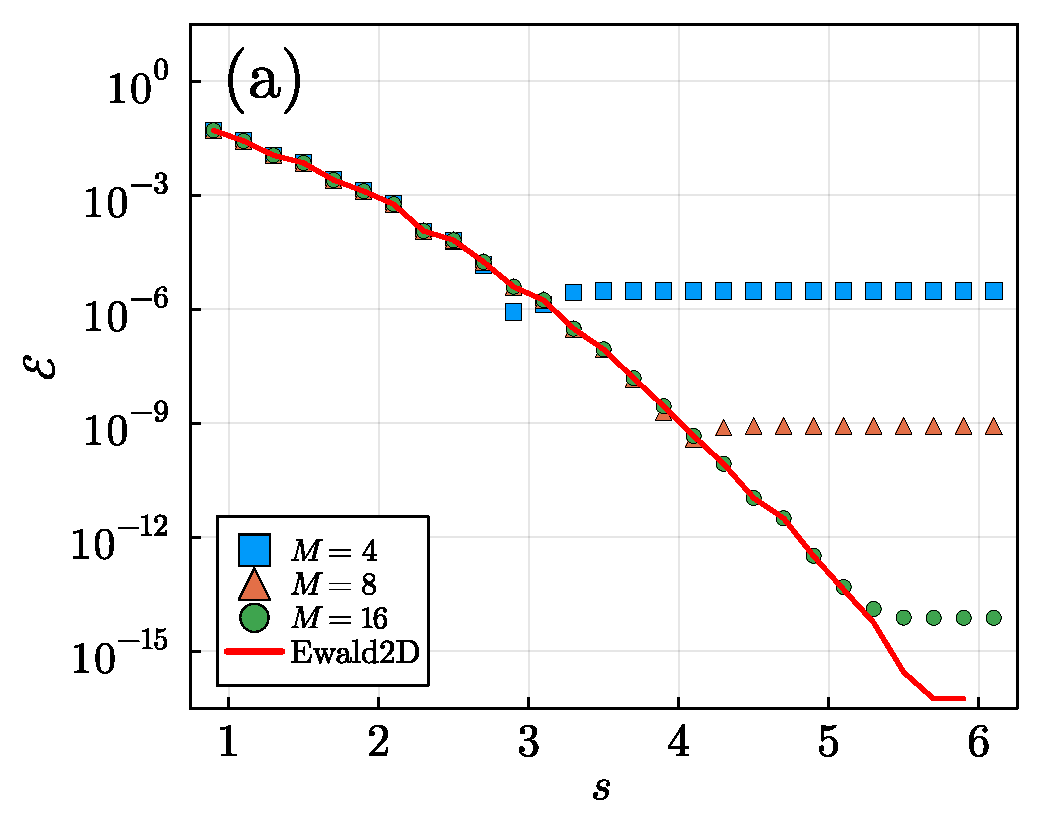
\includegraphics[width=0.48\textwidth]{figs/fig_error_fixn.pdf}
	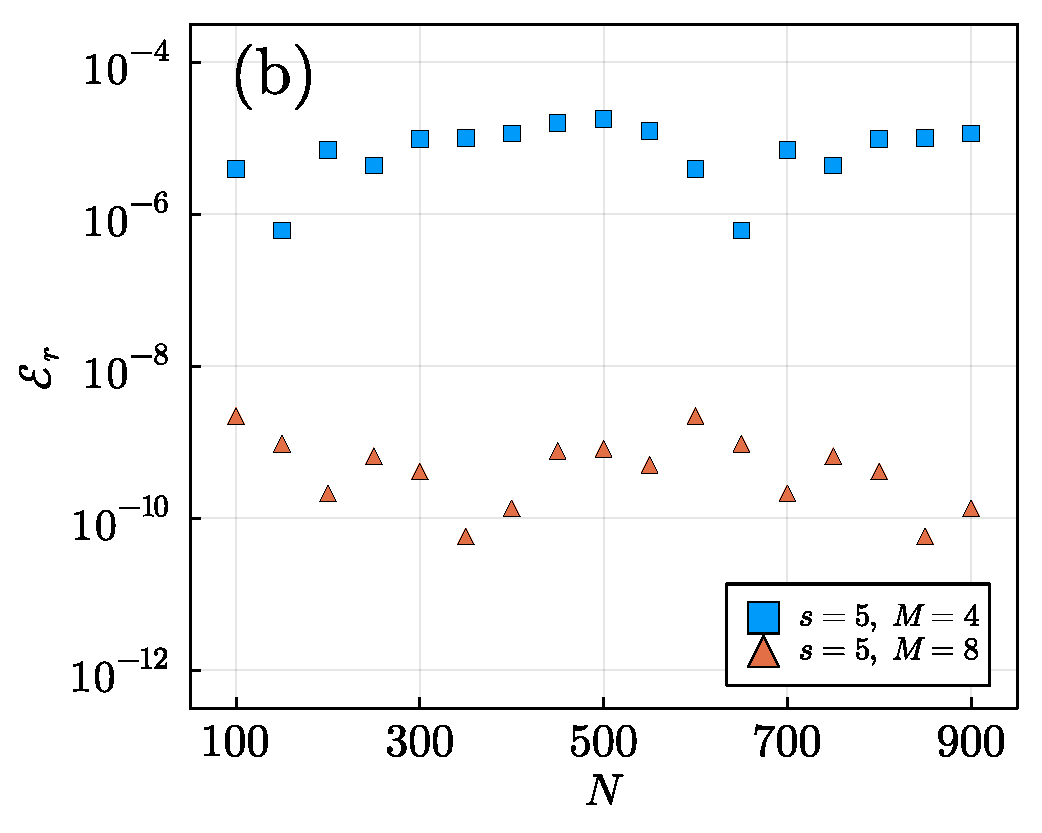
\includegraphics[width=0.48\textwidth]{figs/fig_error_N.pdf}
	\caption{
		Accuracy in the electrostatic energy by the SOEwald2D method. (a): absolute error as a function of $s$; (b): relative error as a function of total number of ions $N$ with fixed ion density $\rho_{s}$. Results with different number of exponentials $M$ are considered. 
	}
	\label{fig:error_fixn}
\end{figure}

\begin{figure}[ht]
	\centering
	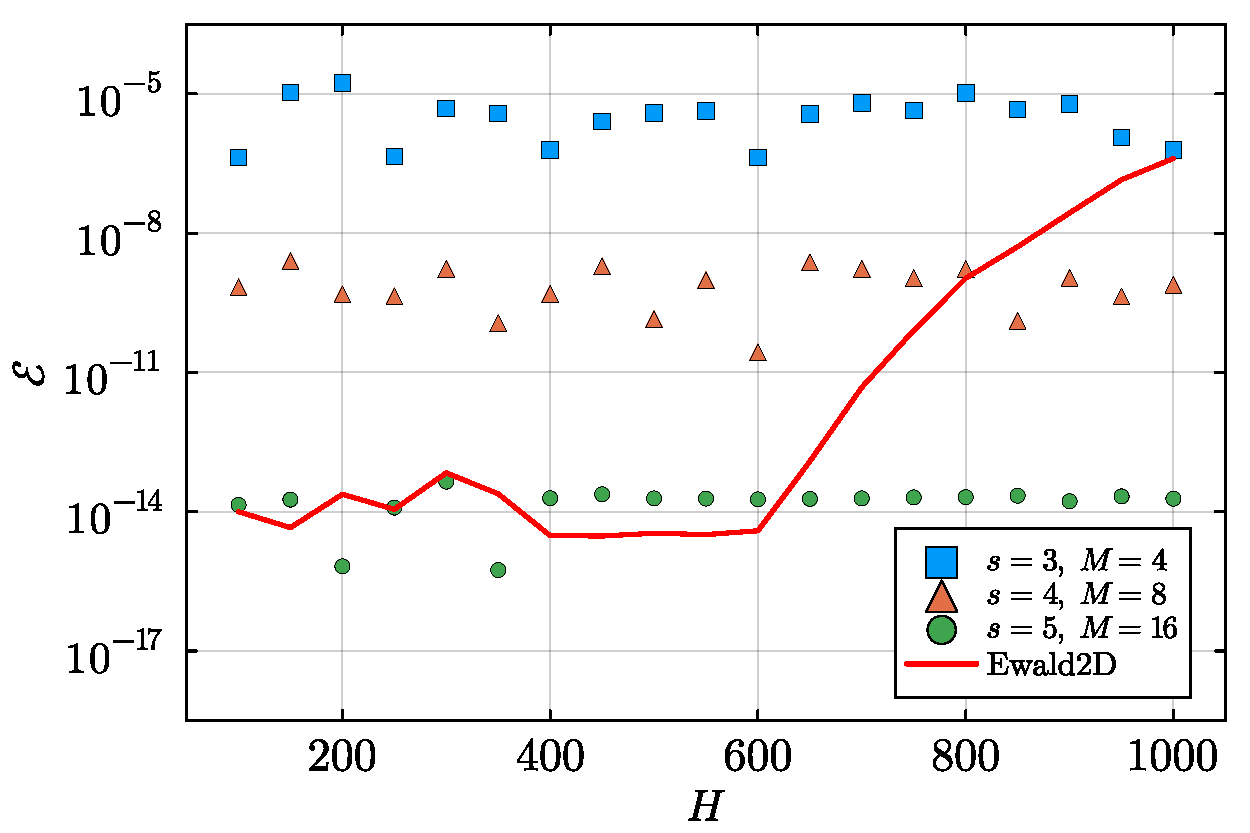
\includegraphics[width=0.6\textwidth]{figs/fig_error_Lz.pdf} 
	\caption{
		The absolute error in electrostatic energy is evaluated for the SOEwald2D method using three sets of parameters, as well as for the Ewald2D method with $s=5$, as a function of the system's thickness $H$. 
		% The system consists of $100$ uniformly distributed particles, with dimensions $L_x=L_y=100$ along the periodic dimensions. The Ewald parameter is set to $\alpha = 0.1$.
	}
	\label{fig:error_Lz}
\end{figure}

As discussed at the end of Section~\ref{sec::ewald2d}, one notable drawback of the original Ewald2D method is the occurrence of catastrophic error cancellation when the size of the non-periodic dimension increases. 
To quantify this effect, one shall study the absolute error in electrostatic energy as a function of $H$. 
The Ewald2D truncation parameter~$s= 3, 4, 5$ are chosen for~$M = 4, 8, 16$, respectively, to obtain optimal accuracy as is guided by Figure~\ref{fig:error_fixn} (a).
The system consists of $100$ uniformly distributed particles, with dimensions $L_x = L_y = 100$ along the periodic dimensions, and the Ewald parameter is set to be $\alpha = 0.1$.
A double-precision floating-point (FP64) arithmetic for both the Ewald2D and SOEwald2D methods is employed, while the reference solution is obtained using the Ewald2D with a quadruple-precision floating-point (FP128) arithmetic, ensuring a sufficient number of significant digits. 
The results presented in Figure~\ref{fig:error_Lz} clearly illustrate that the error of the Ewald2D method increases rapidly with $H$.
In contrast, the error of the SOEwald2D method remains independent of $H$ for various values of $s$ and $M$, thanks to its stable and well-conditioned summation procedure.

For many existing methods, the accurate evaluation of the forces exert on particles can be strongly influenced by the particle's location in~$z$. 
Due to the uniform convergence of SOE approximation, our method does not suffer from this issue, which is illustrated by two commonly employed examples that have been extensively studied in literature~\cite{lindbo2012fast,de2002electrostatics}. 
In the first example, one considers a system consisting of $50$ anions and $50$ cations arranged in a cubic geometry with a side length of $100$, along with neutral slabs.  
The pointwise error of the force, represented as $\sqrt{\mathscr{E}_{x}^2+\mathscr{E}_{y}^2+\mathscr{E}_{z}^2}$,  is calculated as a function of the particles' $z$-coordinates. 
This evaluation is conducted for various $(s,M)$ pairs, with the Ewald splitting parameter $\alpha=0.1$. 
Figure~\ref{fig:error_ef}(a) clearly demonstrates that the pointwise error in force is independent with its relative position in $z$. 
In the second example, one considers a system of the same size but with two non-neutral slabs. 
The surface charge densities are set as $\sigma_{\mathrm{top}} = \sigma_{\mathrm{bot}} = -0.005$, and the system contains $100$ monovalent cations such that the neutrality condition Eq.~\eqref{eq::chargeneu} is satisfied. 
Figure~\ref{fig:error_ef}(b) indicates that for such non-neutral slabs case, the pointwise error in forces calculated by the SOEwald2D method remains independent with $z$.

\begin{figure}[ht]
	\centering
	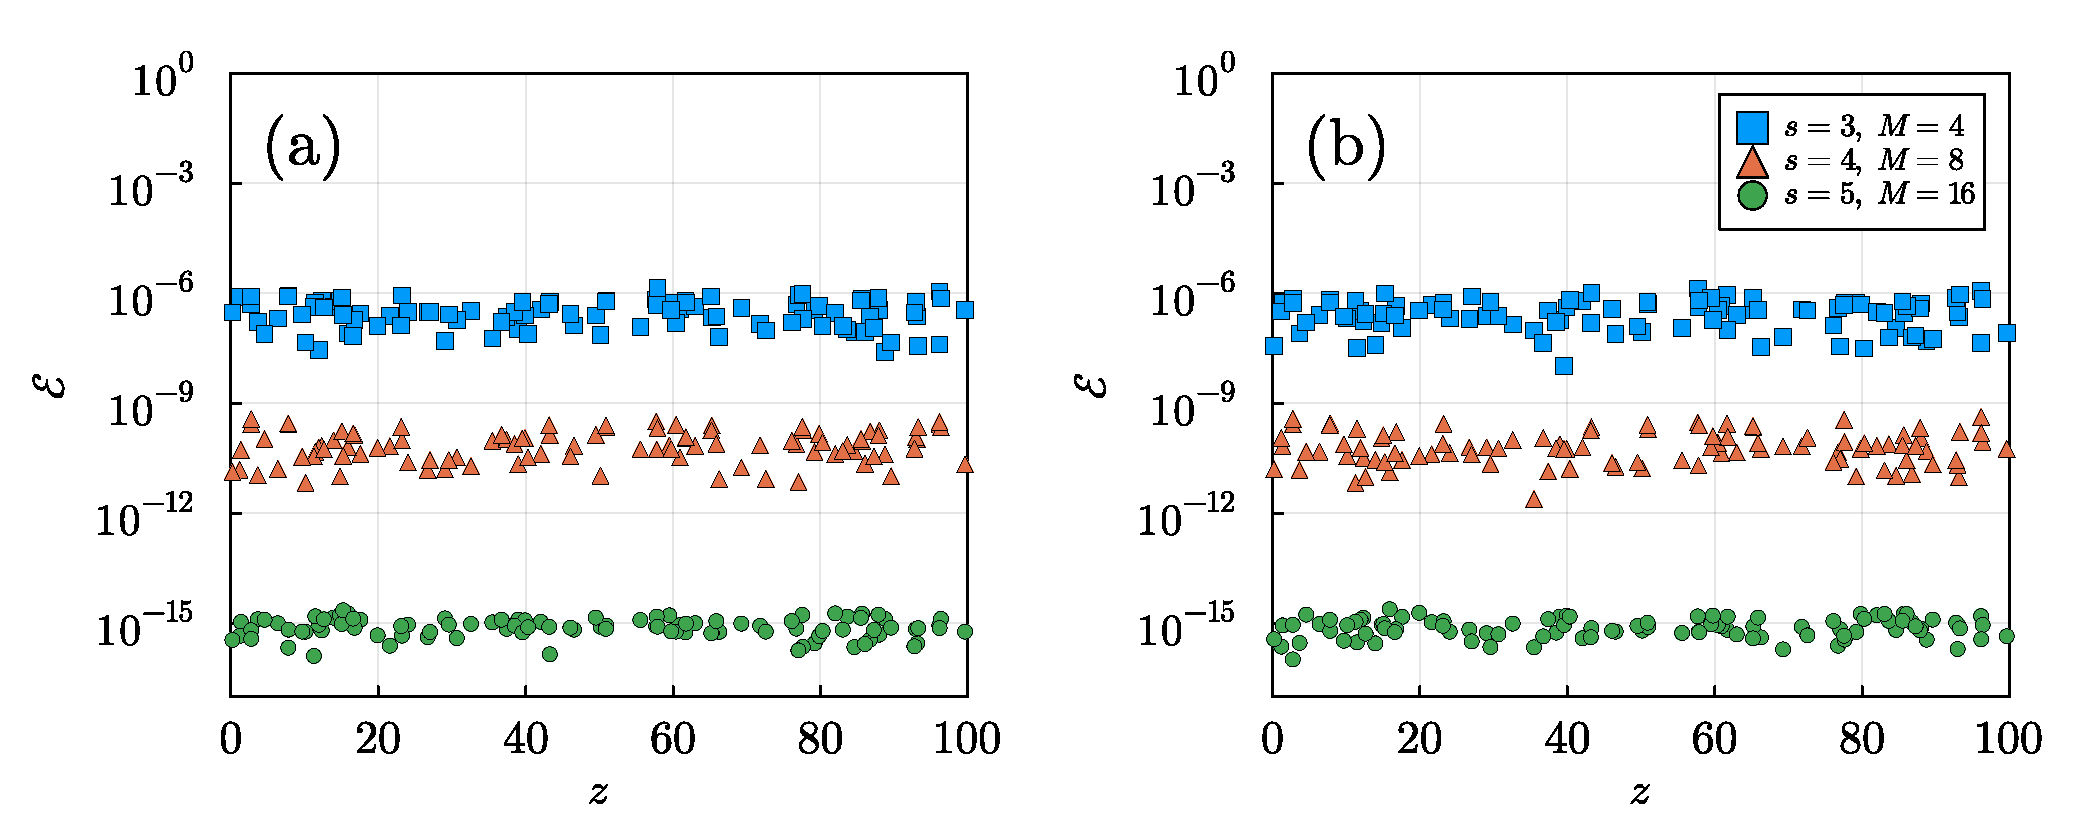
\includegraphics[width=\textwidth]{figs/fig_error_ef.pdf} 
	\caption{
		The absolute error in the pointwise electrostatic forces calculated using the SOEwald2D versus particles' $z$-coordinates. 
		Two different scenarios are considered: (a) uniformly distributed 50 anions and 50 cations and (b) uniformly distributed 100 cations with surface charge densities $\sigma_{\mathrm{top}}= \sigma_{\mathrm{bot}} = -0.005$.
	}\label{fig:error_ef}
\end{figure}

\subsection{Accuracy of the RBSE2D method}\label{subsec::RBSE2D}

In contrast to the deterministic SOEwald2D and Ewald2D methods, the  RBSE2D employs unbiased stochastic approximations and its convergence should be investigated in the sense of ensemble averages, as has been carefully discussed in Sec.~\ref{sec:rbm}. 
%The intuition why such stochastic methods work is that the effect of random approximations accumulates in time. Since the random approximation is unbiased, the random errors will roughly cancel out over time. This ``law of large numbers'' type mechanism in time then makes the random method work. 
Therefore, we conduct a series of MD simulations to validate the accuracy of the ensemble averaged equilibrium and dynamical quantities such as particles' concentrations and  mean-squared displacements (MSD) computed using the RBSE2D algorithm.

\begin{figure}[ht]
	\centering
	\begin{minipage}[c]{\textwidth}
		\centering
		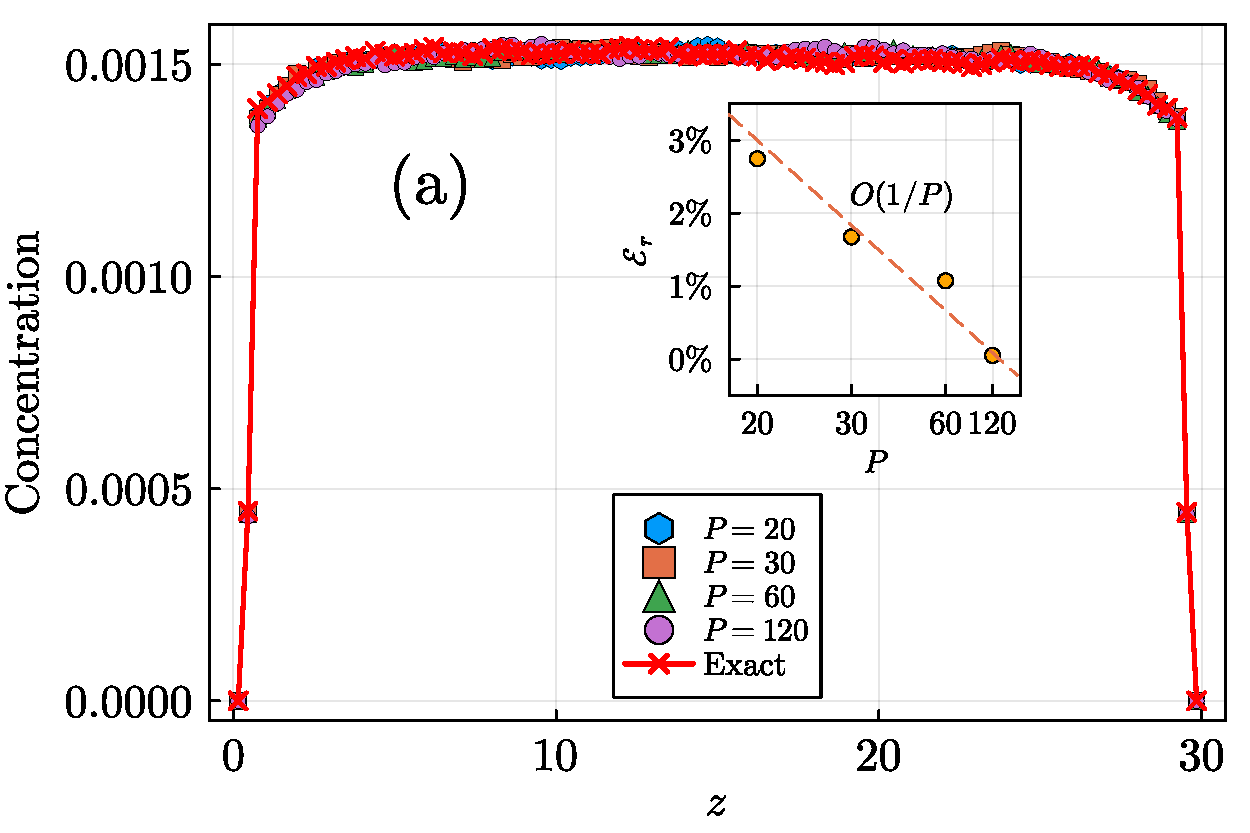
\includegraphics[width=0.6\textwidth]{figs/hist_norm.pdf}
		\label{fig:compare}
	\end{minipage} \\
	\begin{minipage}[c]{\textwidth}
		\centering
		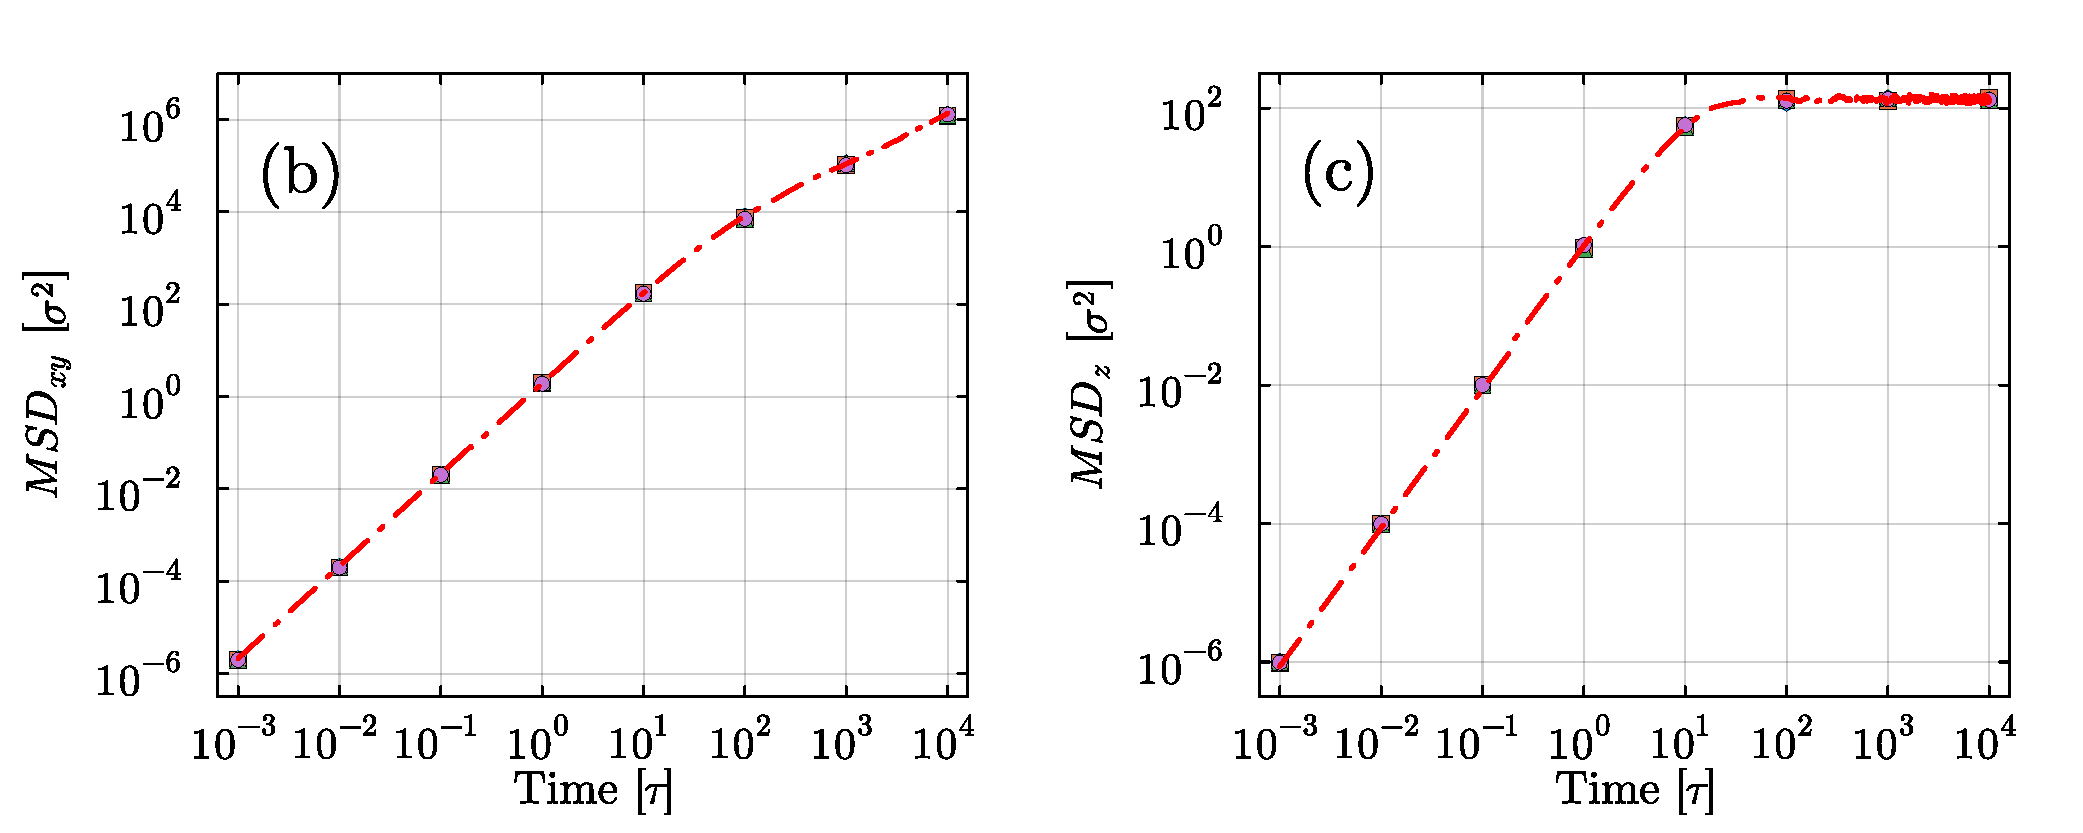
\includegraphics[width=\textwidth]{figs/msd_norm.pdf} 
		\label{fig:msd_norm}
	\end{minipage} 
	\caption{
		(a) The concentration of cations along $z$, with subplot indicating the convergence in the relative error of the average electrostatic energy as a function of batch size~$P$; (b) and (c) the MSD profiles in~$xy$ and~$z$ against time for a $1:1$ electrolyte confined by neutral slabs. 
		Results by using different batch sizes $P=20, 30, 60, 120$ are shown. 
	}
	\label{fig:norm}
\end{figure}

The first benchmark example is a coarse-grained MD simulation of  $1:1$ electrolytes in the NVT ensemble. 
Following the primitive model~\cite{frenkel2023understanding}, ions are represented as soft spheres with diameter $\sigma$ and mass $m$, interacting through the Coulomb potential and a purely repulsive shifted-truncated Lennard Jones (LJ) potential. 
The LJ potential is given by
\begin{equation}
	U_{\text{LJ}}(r) = 
	\begin{cases}
		4 \epsilon \left[ \left(\dfrac{\sigma}{r}\right)^{12}-\left(\dfrac{\sigma}{r}\right)^6 + \dfrac{1}{4}\right],\quad & r < r_{\text{LJ}}, \\
		0, & r \geq r_{\text{LJ}},
	\end{cases}
\end{equation}
where $r_{\text{LJ}} = 2^{1/6} \sigma$ is the LJ cutoff, $\epsilon = k_B T$ is the coupling strength, $k_B$ is the Boltzmann constant, and $T$ is the external temperature. 
The simulation box has dimensions $L_x = L_y = 100 \sigma$ and $H = 30 \sigma$, where the ions confined within the central region by purely repulsive LJ walls located at $z = 0$ and $z = 30 \sigma$ with $\epsilon_{\text{wall}} = \epsilon_{\text{LJ}}$ and $\sigma_{\text{wall}} = 0.5 \sigma$. 
The system contains $218$ cations and anions, and both two walls are neutral. 
The simulation is performed with the time step~$\Delta=0.001\tau$, where~$\tau = \sqrt{m \sigma^2 / \eps_{\text{LJ}}}$ denotes the LJ unit of time. 
The temperature is maintained by using a Nos\'e-Hoover thermostat~\cite{frenkel2023understanding} with relaxation times $0.1\tau$, fluctuating near the reduce external temperature $T=1$.
The system is first equilibrated for~$5 \times 10^5$ steps, and the production phase lasts another~$1 \times 10^7$ steps. 
The configurations are recorded every $100$ steps for statistics. Results produced by the SOEwald2D method with parameters $\alpha=0.1$, $s=4$, and $M=8$ serve as the reference solution, where $\varepsilon\sim 10^{-8}$.

The ion concentration along the $z$-direction is measured, and presented in Figure~\ref{fig:norm}. 
For the RBSE2D method, simulations with varying batch sizes $P$ are performed, while keeping other parameters fixed at $\alpha = 0.3$, $s=4$, and $M=8$. 
It is observed that the results for all choices of $P$ are in excellent agreement with those obtained using the accurate SOEwald2D method. 
Furthermore, one evaluates the MSDs along both the periodic dimensions (Figure~\ref{fig:norm}(a)) and the non-periodic dimension (Figure~\ref{fig:norm}(b)), which describe the particles' anisotropic dynamic properties across a wide range of time scales. 
The RBSE2D methods for all $P$ yield almost identical MSD results as the SOEwald2D method. 
The confinement effect in $z$ leads to a $MSD_z$ profile that clearly indicates a subdiffusion, while $MSD_{xy}$ exhibits a normal diffusion process. 
Clearly, the RBSE2D method successfully captures this anisotropic collective phenomenon.


\begin{figure}[ht]
	\centering
	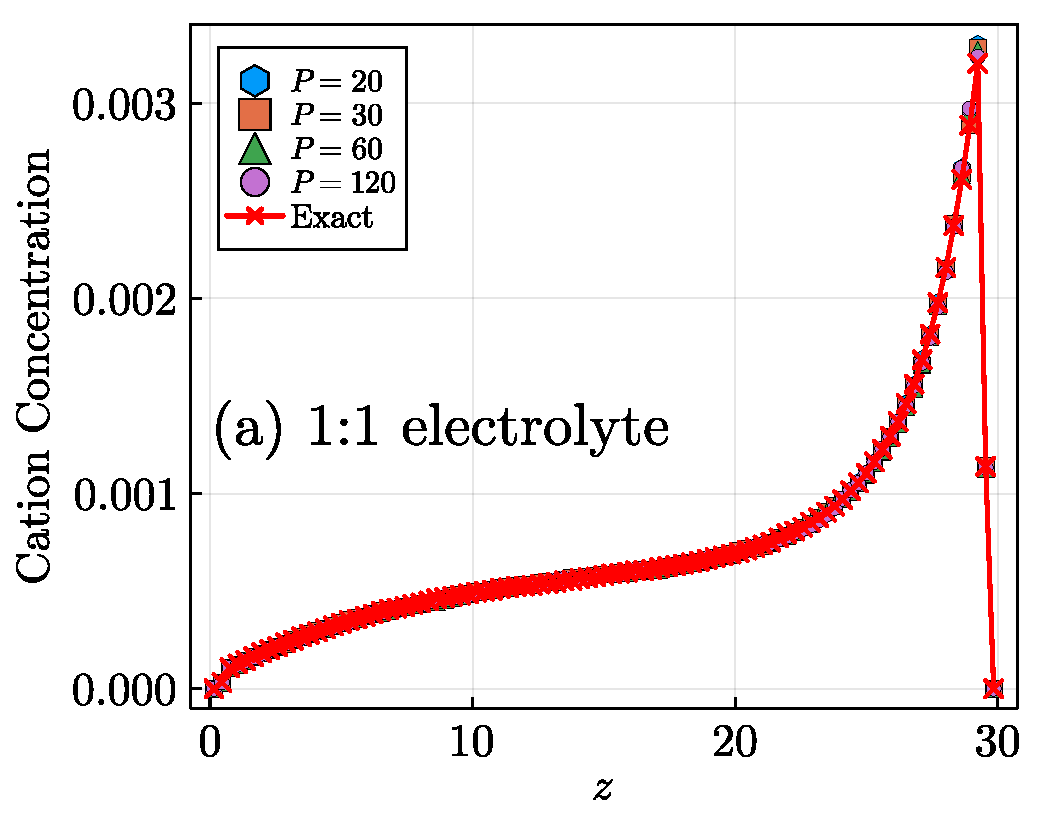
\includegraphics[width=0.49\textwidth]{figs/hist_Ez.pdf} 
	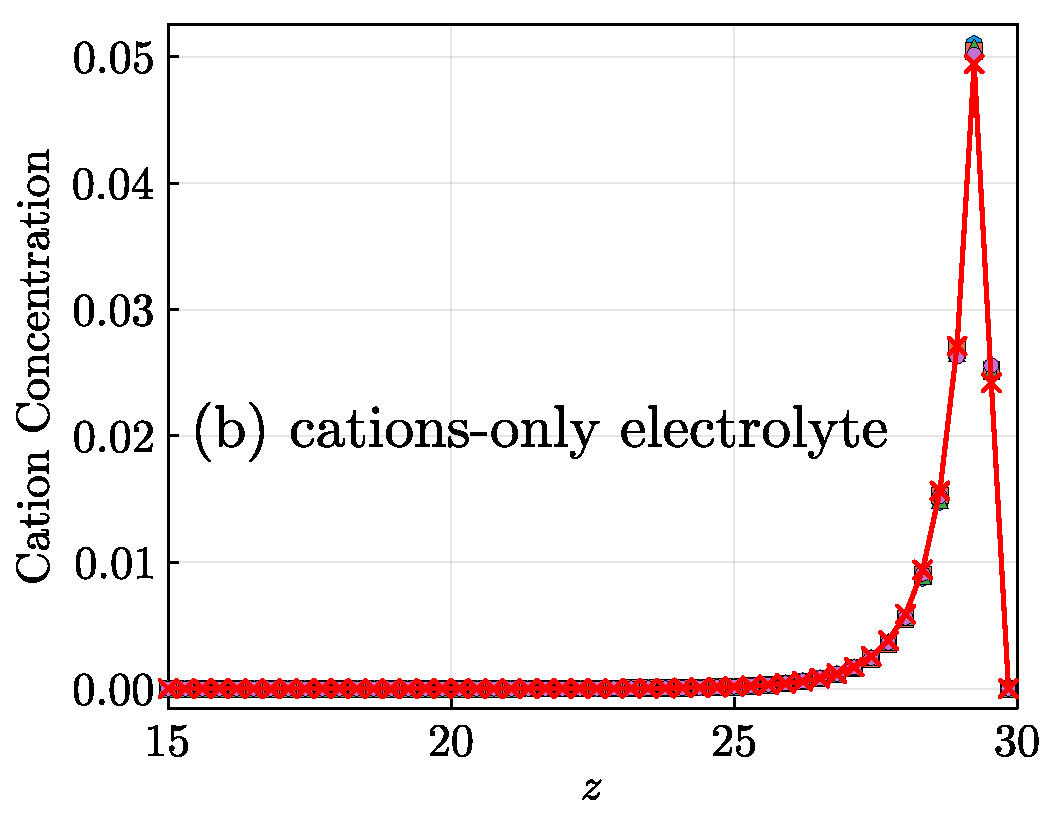
\includegraphics[width=0.49\textwidth]{figs/hist_cation.pdf}
	\caption{
		Concentration of cations in $z$ for (a) a $1:1$ electrolyte confined between two charged slabs and (b) a cations-only system confined between two slabs, one of which is charged to neutralize the system. 
	}
	\label{fig:Ez_density}
\end{figure}


To assess the performance of our RBSE2D method for systems with non-neutral slabs, one studies
a $1:1$ electrolyte containing~$218$ anions and~$218$ cations with~$q = \pm 1$, and with surface charge densities $\sigma_{\mathrm{bot}}=0.0218$ and~$\sigma_{\mathrm{top}}=-0.0218$. The simulation box is set to be $L_x = L_y = 100 \sigma$ and $H = 30 \sigma$.
The resulting equilibrium concentration of cations is shown in Figure~\ref{fig:Ez_density}(a), indicating that results of RBSE2D method with different batch sizes are in good agreement with that of the reference SOEwald2D method. 
% The subplot of Figure~\ref{fig:Ez_density}(a) also depicts the convergence as the batch size $P$ increases, which is consistent with our analysis.

We further investigate the most challenging scenario for a system with free cations only, which are confined by non-neutral slabs, so that boundary layers can form at the vicinity of the slabs. 
In particular, the system consists of $436$ monovalent cations and is confined by slabs with surface charge densities $\sigma_{\mathrm{bot}}=0$ and $\sigma_{\mathrm{top}}=-0.0436$ to ensure overall charge neutrality. The concentration of free ions is depicted in Figure~\ref{fig:Ez_density}(b), exhibiting excellent agreement with the results obtained using the SOEwald2D method. 
% The subplot in Figure~\ref{fig:Ez_density}(b) also demonstrates the expected convergence of the RBSE2D method as the batch size increases. 
These findings indicate that choosing a small batch size $P\sim\mathcal O(1)$ is sufficient for generating accurate MD results by using the RBSE2D method.

\subsection{CPU performance}
The CPU performance comparisons among the SOEwald2D, RBSE2D, and the original Ewald2D methods are conducted for MD simulations of $1:1$ electrolyte systems with varying system sizes. 
All calculations are performed on a Linux system equipped with an Intel Xeon Platinum 8358 CPU (2.6 GHz, 1 single core); and by using a self-developed package developed in Julia language. 
To ensure a fair comparison, we maintain the same accuracy across all methods. We fix $s=4$ and set $M=8$ for the SOE approximation, resulting in errors at~$\sim10^{-8}$ for both the Ewald2D and SoEwald2D methods. %as shown in Figure~\ref{fig:error_fixn}(a).
Subsequently, we set the batch size as $P=120$ for the RBSE2D method, with which the RBSE2D-based MD simulations achieve the same accuracy as the SOEwald2D method, as has been illustrated in the previous results.
%It is remarked that the Ewald2D, SOEwald2D, and RBSE2D methods scale as $\mathcal{O}(s^2)$, $\mathcal{O}(s^2 M)$, and $\mathcal{O}(s^2 M P)$, respectively.
Finally, for each of the methods, the Ewald splitting parameter $\alpha$ is always adjusted to achieve optimal efficiency.
The CPU time comparison results are summarized in Figure~\ref{fig:times_compare}. 
It is evident that the CPU cost of the Ewald2D, SOEwald2D, and RBSE2D methods scale as $\mathcal{O}(N^2)$, $\mathcal{O}(N^{7/5})$, and $\mathcal{O}(N)$, respectively, which is consistent with our complexity analysis. 
Remarkably, the RBSE2D method demonstrates a significant speedup of $3\times 10^3$-fold compared to the Ewald2D for a system with $N=10^{4}$ particles, enabling large-scale MD simulations on a single core.

An additional observation is regarding the memory consumption and data input/output (I/O) on the maximum system size that can be simulated using the same computational resources. 
In Figure~\ref{fig:times_compare}, it is demonstrated that when utilizing a single CPU core, the Ewald2D and SOEwald2D methods are limited to simulating system sizes of up to about $3 \times 10^4$ and $3 \times 10^5$ particles, respectively. 
In contrast, the RBSOEwald method can handle systems containing about $5 \times 10^6$ particles. 
This is attributed to the reduced number of interacting neighbors that need to be stored in the RBSE2D algorithm, allowing a much smaller real space cutoff $r_c$. 
This significant saving in memory consumption is achieved by the algorithm developed in this study, highlighting its potential as an effective algorithm framework for large-scale simulations of quasi-2D Coulomb systems.

\begin{figure}[ht]
	\centering
	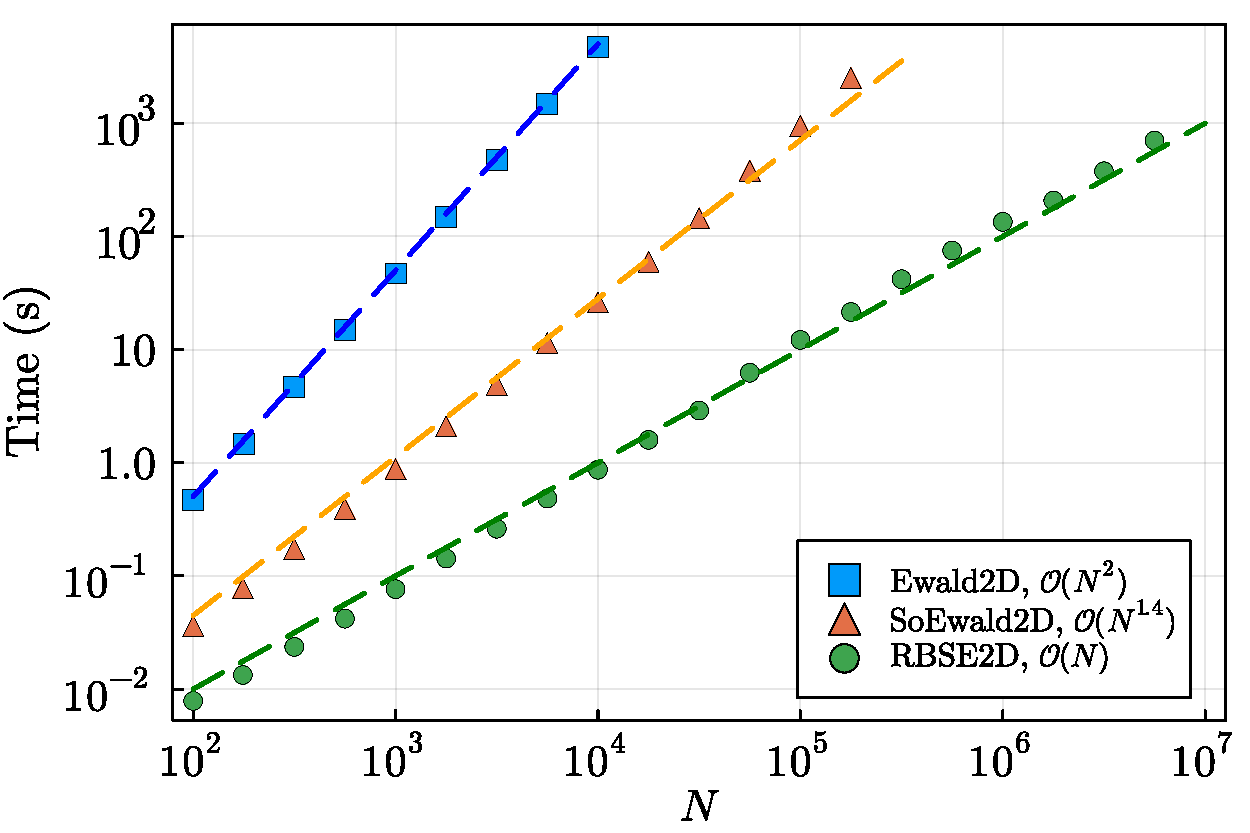
\includegraphics[width=0.6\textwidth]{figs/times_compare.pdf} 
	\caption{
		The CPU time cost for the Ewald2D, SOEwald2D, and RBSE2D methods versus the number of particles $N$, with fixed particle density $\rho_s$. 
	}
	\label{fig:times_compare}
\end{figure}